
\section{Device Frabrication}

\subsection{PDMS channels}

\begin{figure}[h]
    \centering
    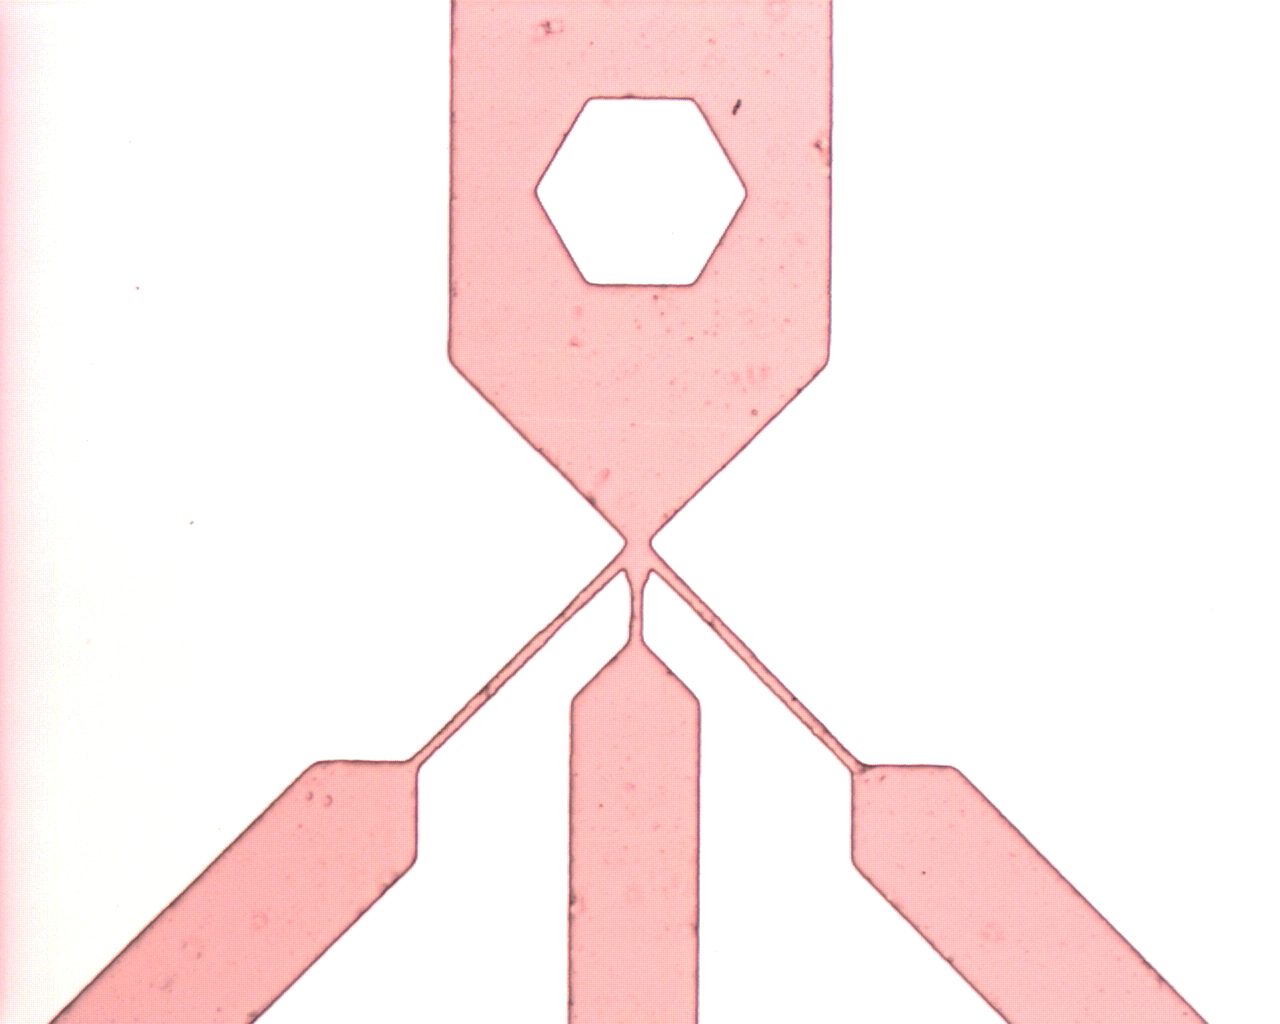
\includegraphics[width=\textwidth]{images/su8_results.png}
    \caption{SU-8 photoresist on the master mold.}
    \label{fig:su8_results}
\end{figure}

\begin{figure}[h]
    \centering
    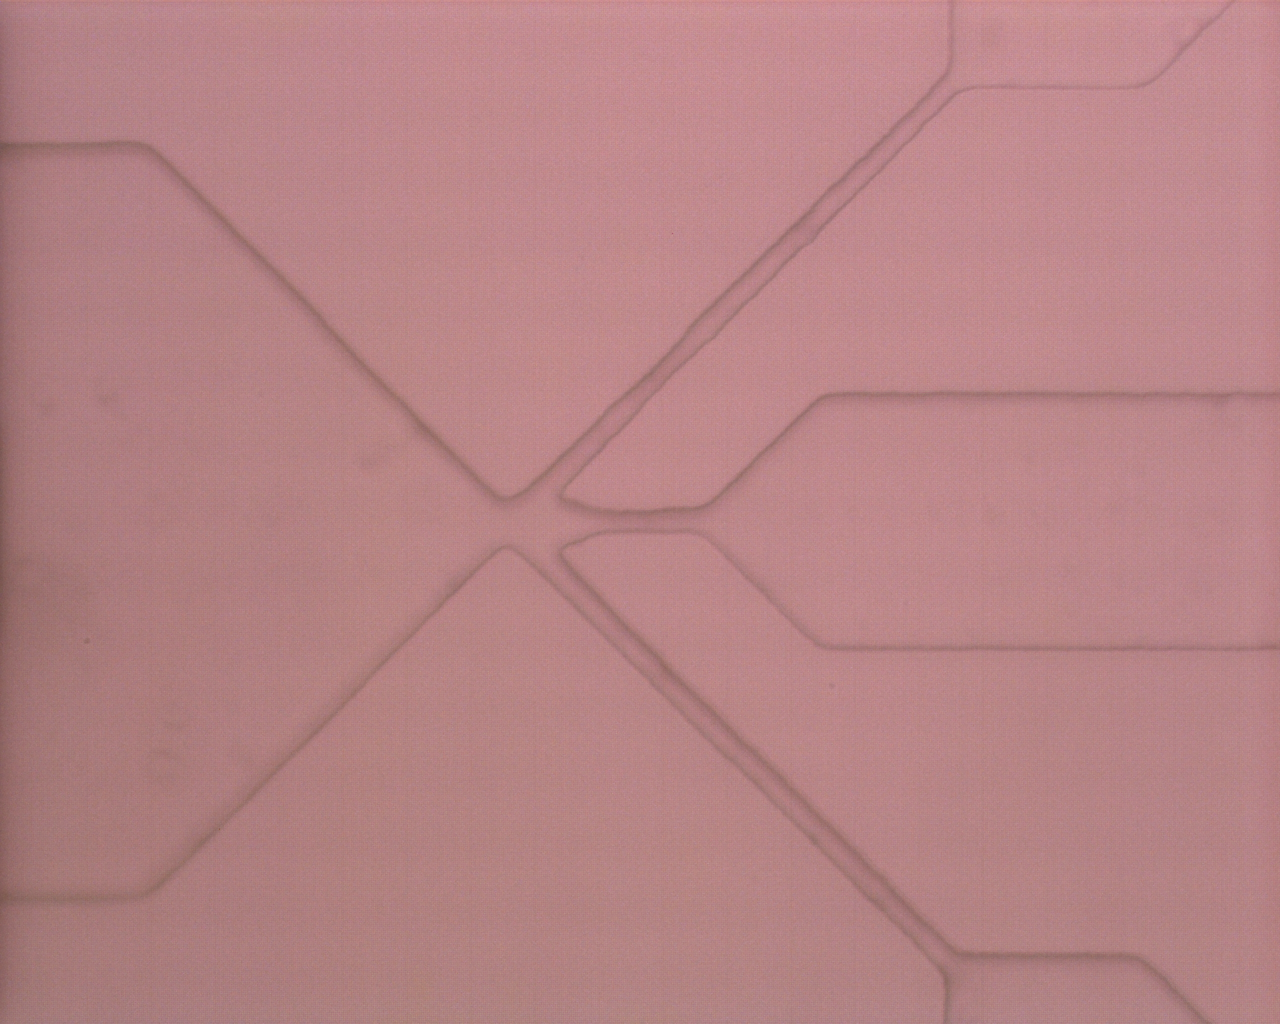
\includegraphics[width=\textwidth]{images/PDMS_channels.png}
    \caption{PDMS cast from the master mold.}
    \label{fig:pdms_results}
\end{figure}

\begin{figure}[h]
    \centering
    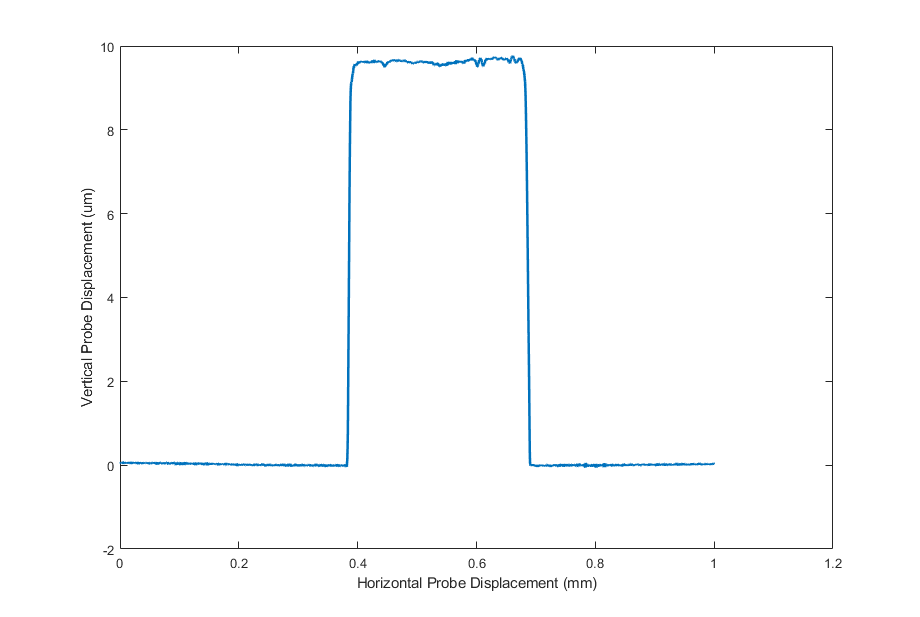
\includegraphics[width=\textwidth]{images/300umWideChannel.png}
    \caption[Surface profile of a 300 micron wide channel on the SU-8 master mold.]{Surface profile of a 300 micron wide channel on the SU-8 master mold. The profile was captured with the Ambios XP-1 profilometer. The profilometer recorded a channel height of 9.6 microns.}
    \label{fig:profilometer_300um_channel}
\end{figure}

\begin{figure}[h]
    \centering
    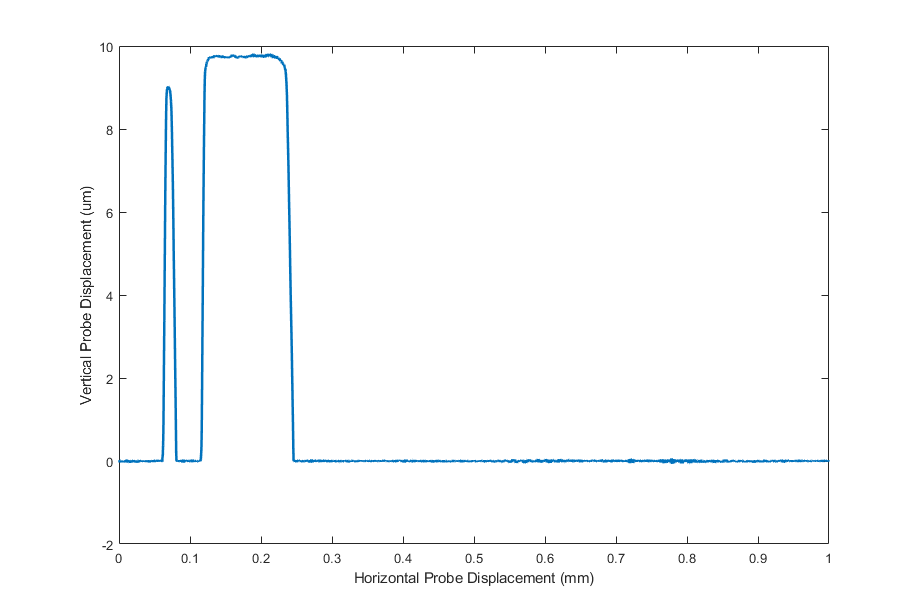
\includegraphics[width=\textwidth]{images/10umWideAndSidewaysThrough100umWide.png}
    \caption[Surface profile of a 10 micron and 100 micron wide channel on the SU-8 master mold.]{Surface profile of a 10 micron and 100 micron wide channel on the SU-8 master mold. The profile was captured with the Ambios XP-1 profilometer. The data depicts the 100 micron channel as about 140 microns wide since it crossed the channel at 45$^\circ$ The profilometer recorded a channel height of 9 and 9.6 microns for the 10 micron and 100 micron channels respectively.}
    \label{fig:profilometer_10um_channel_100um_sideways}
\end{figure}


\FloatBarrier


\subsection{Electrode Fabrication}

\begin{figure}[h]
    \centering
    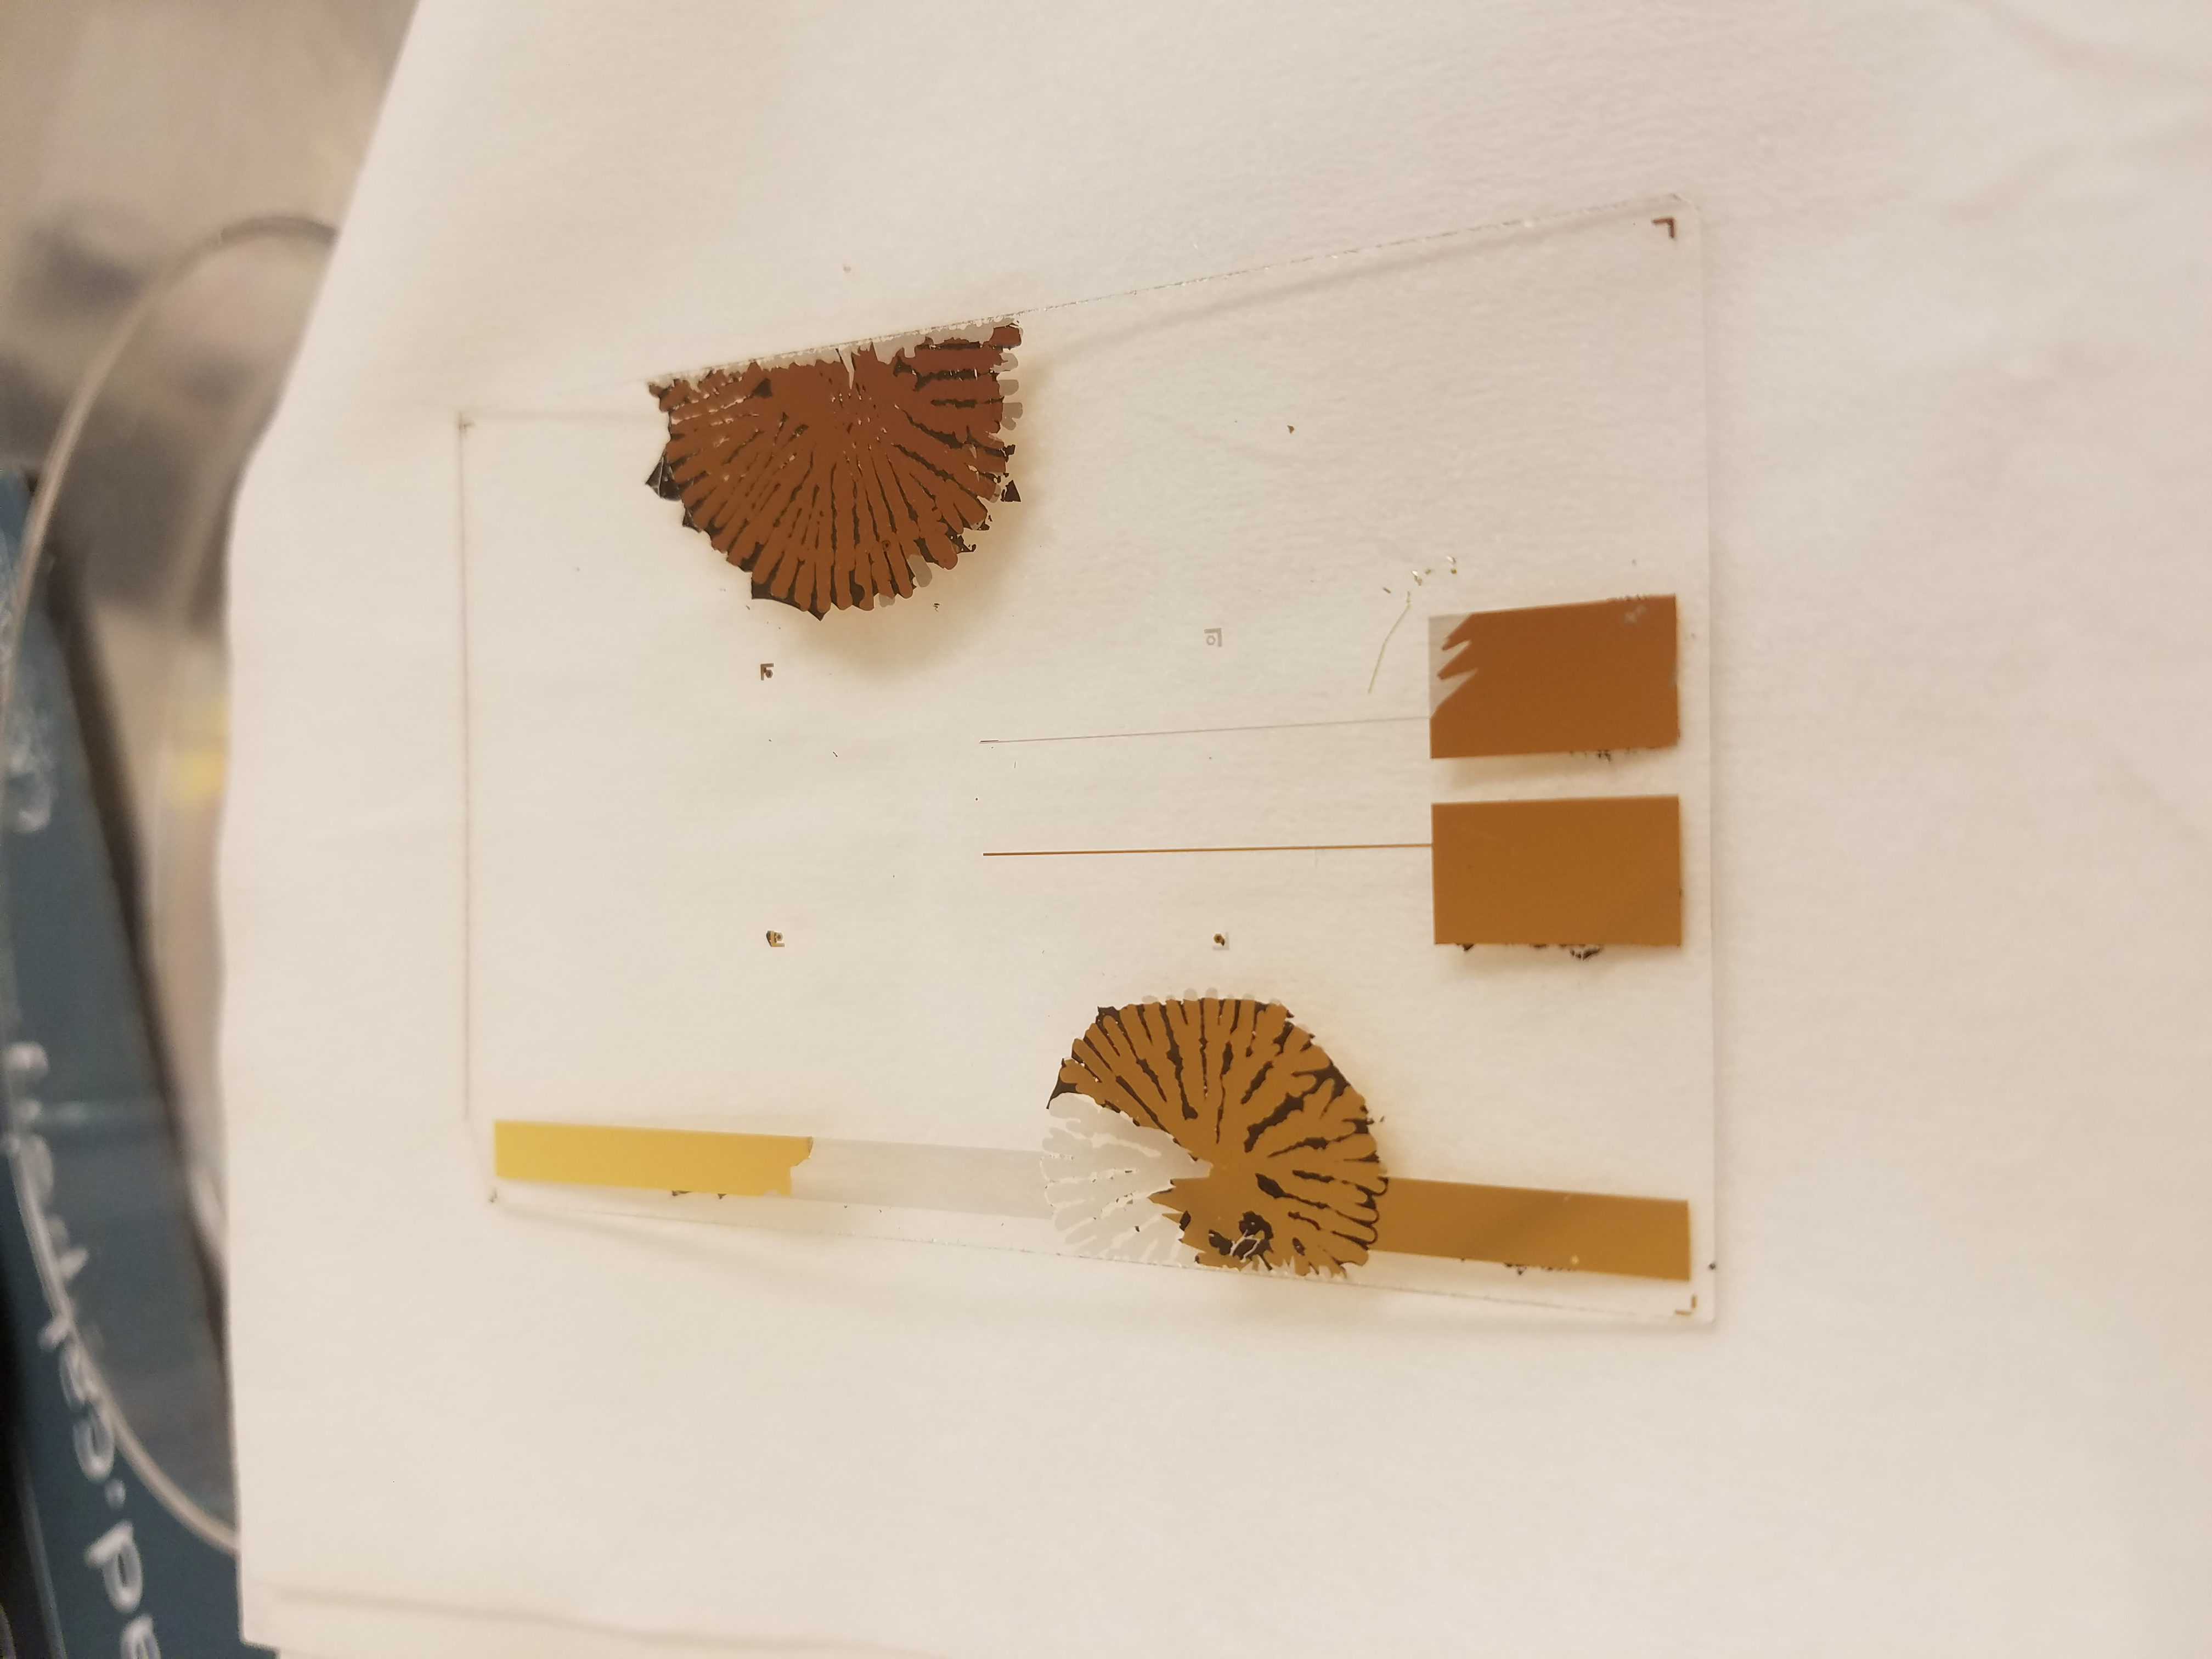
\includegraphics[width=\textwidth]{images/adhesion_issues.jpg}
    \caption{Electrode fabrication failure demonstrating two modes of failure: the ?? photoresist failed to properly adhere to the glass surface manifesting as two anomalous flower patterns, and poor adhesion of the deposited gold to the first chrome layer as evident by gold-stripped leads.}
    \label{fig:failed_electrode_macro}
\end{figure}

\begin{figure}[h]
    \centering
    \begin{subfigure}[b]{0.45\textwidth}
        \centering
        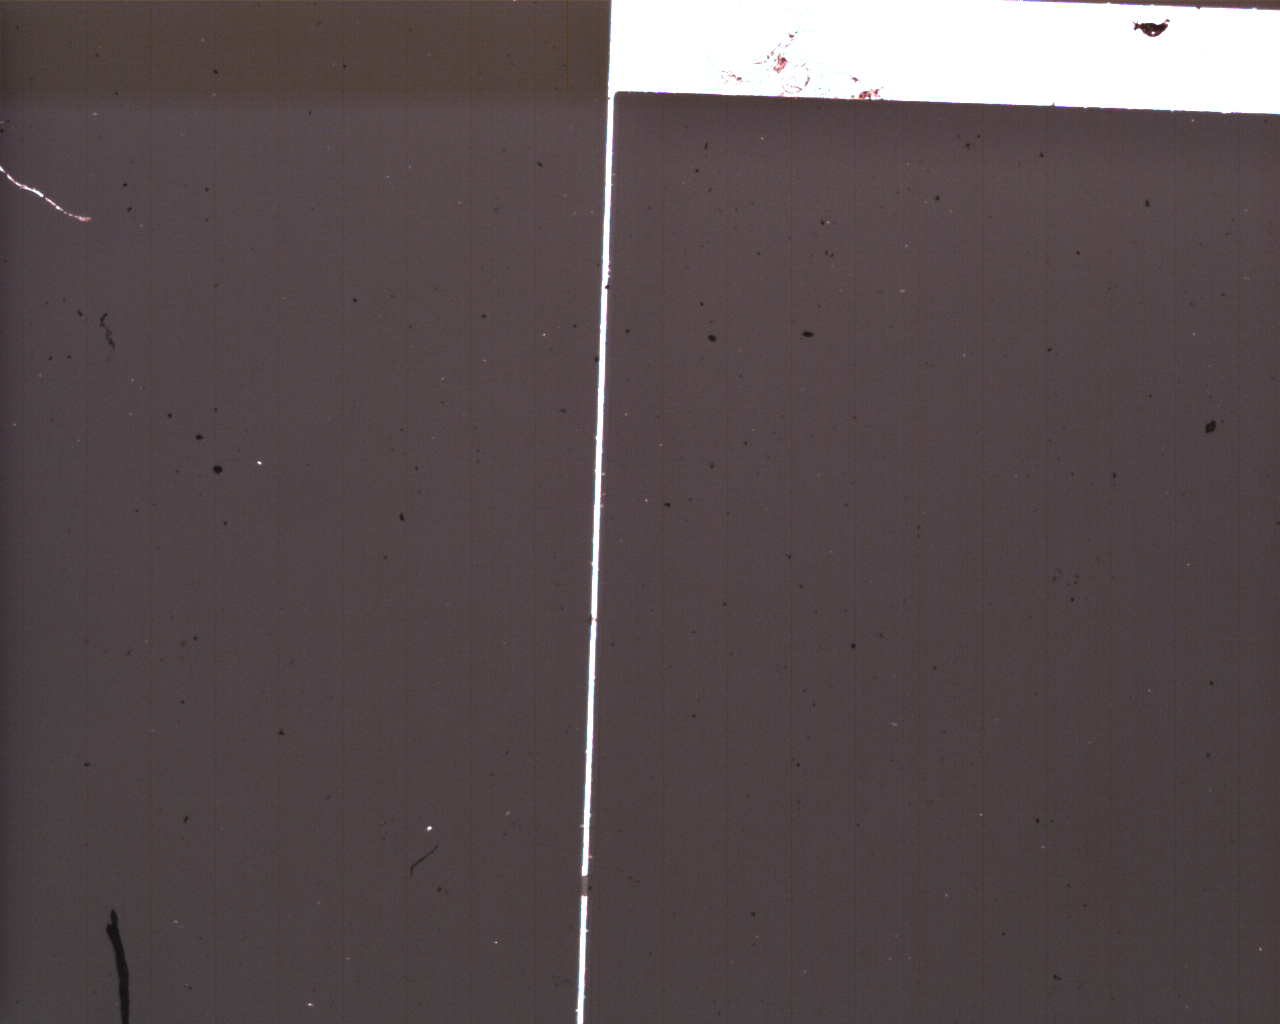
\includegraphics[width=\textwidth]{images/electrodeFailureChunkBreak.png}
        \caption{Impedance magnitude and phase}
    \end{subfigure}
    \hfill
    \begin{subfigure}[b]{0.45\textwidth}
        \centering
        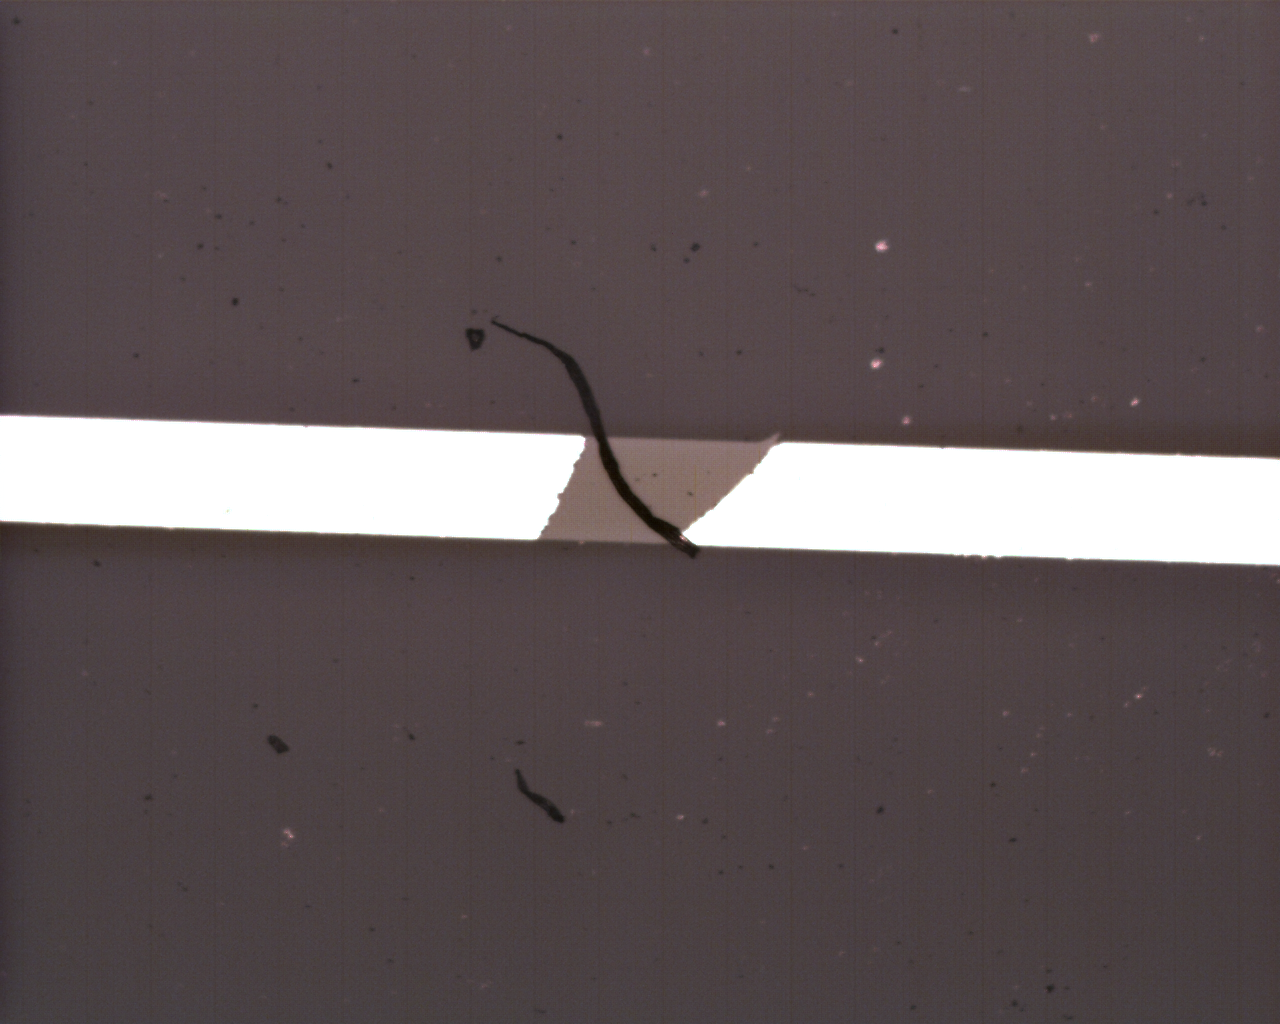
\includegraphics[width=\textwidth]{images/electrodeFailureChunkBreakZoomed.png}
        \caption{Real and imaginary impedance}
    \end{subfigure}
    \\
    \vspace{0.1 in}
    \begin{subfigure}[b]{0.45\textwidth}
        \centering
        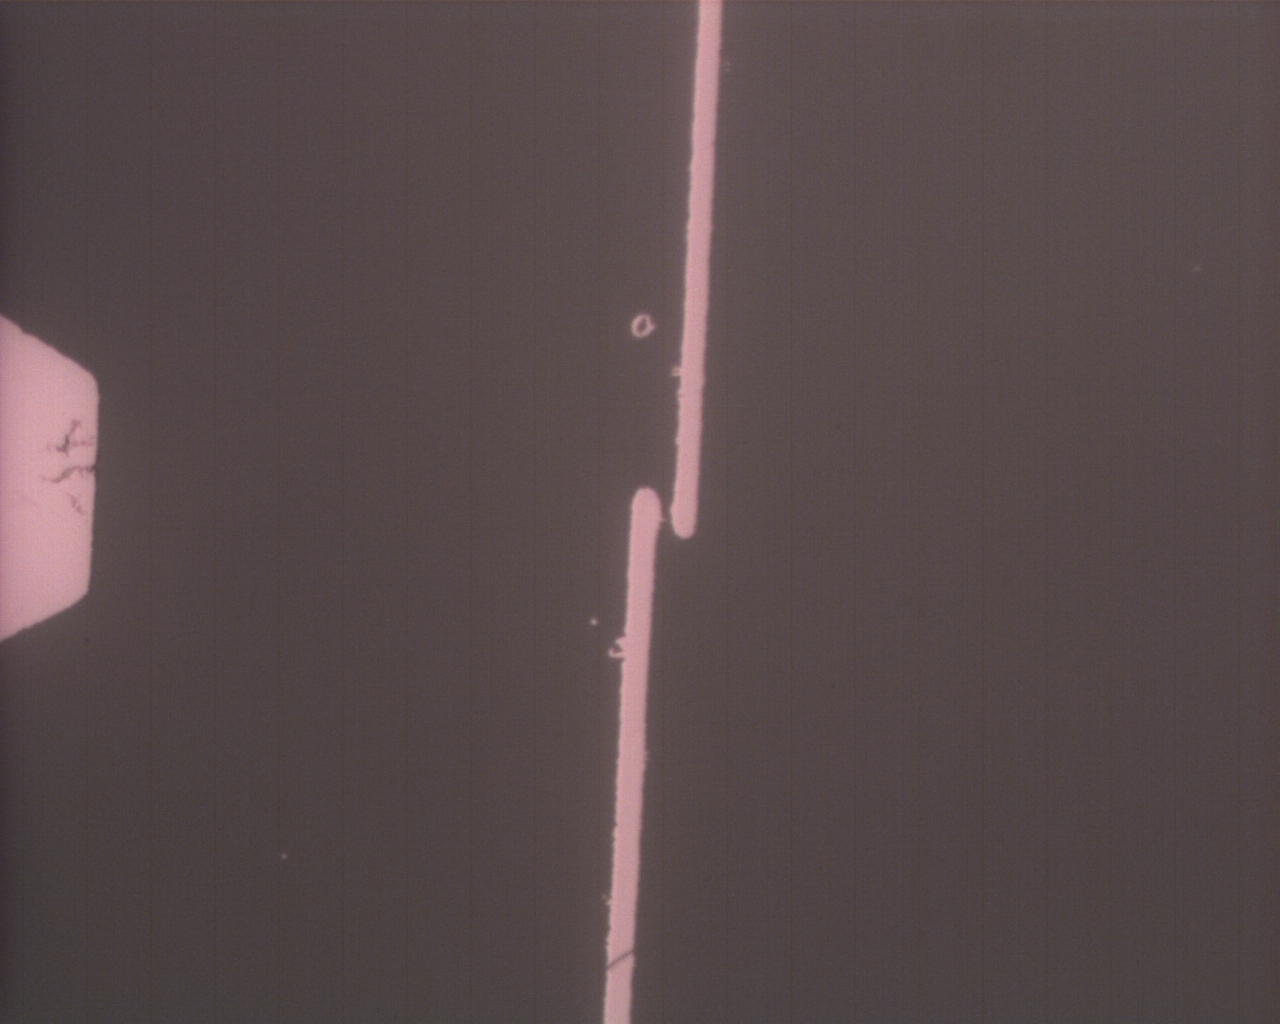
\includegraphics[width=\textwidth]{images/electrodeFailureThinBreak.png}
        \caption{Nyquist plot}
    \end{subfigure}
    \hfill
    \begin{subfigure}[b]{0.45\textwidth}
        \centering
        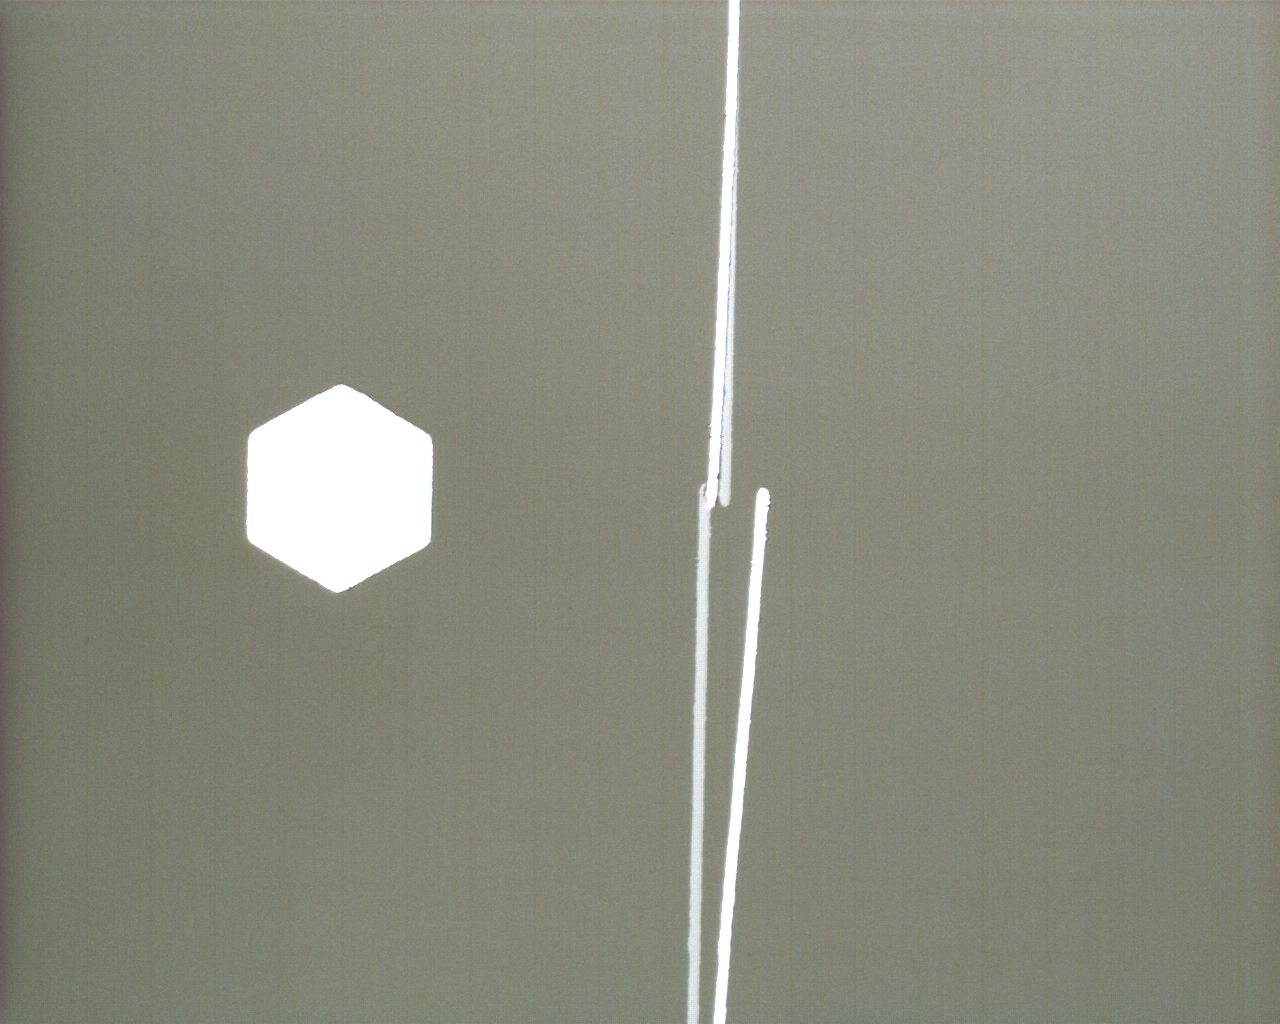
\includegraphics[width=\textwidth]{images/electrodeFailureSlide.png}
        \caption{Clausius Mossotti Factor}
    \end{subfigure}
    \caption{Example plots depicting results of the analytic impedance solution generated by the IS App.}
    \label{fig:failed_elecftrodes_micro}
\end{figure}

\begin{figure}[h]
    \begin{subfigure}[b]{\textwidth}
        \centering
        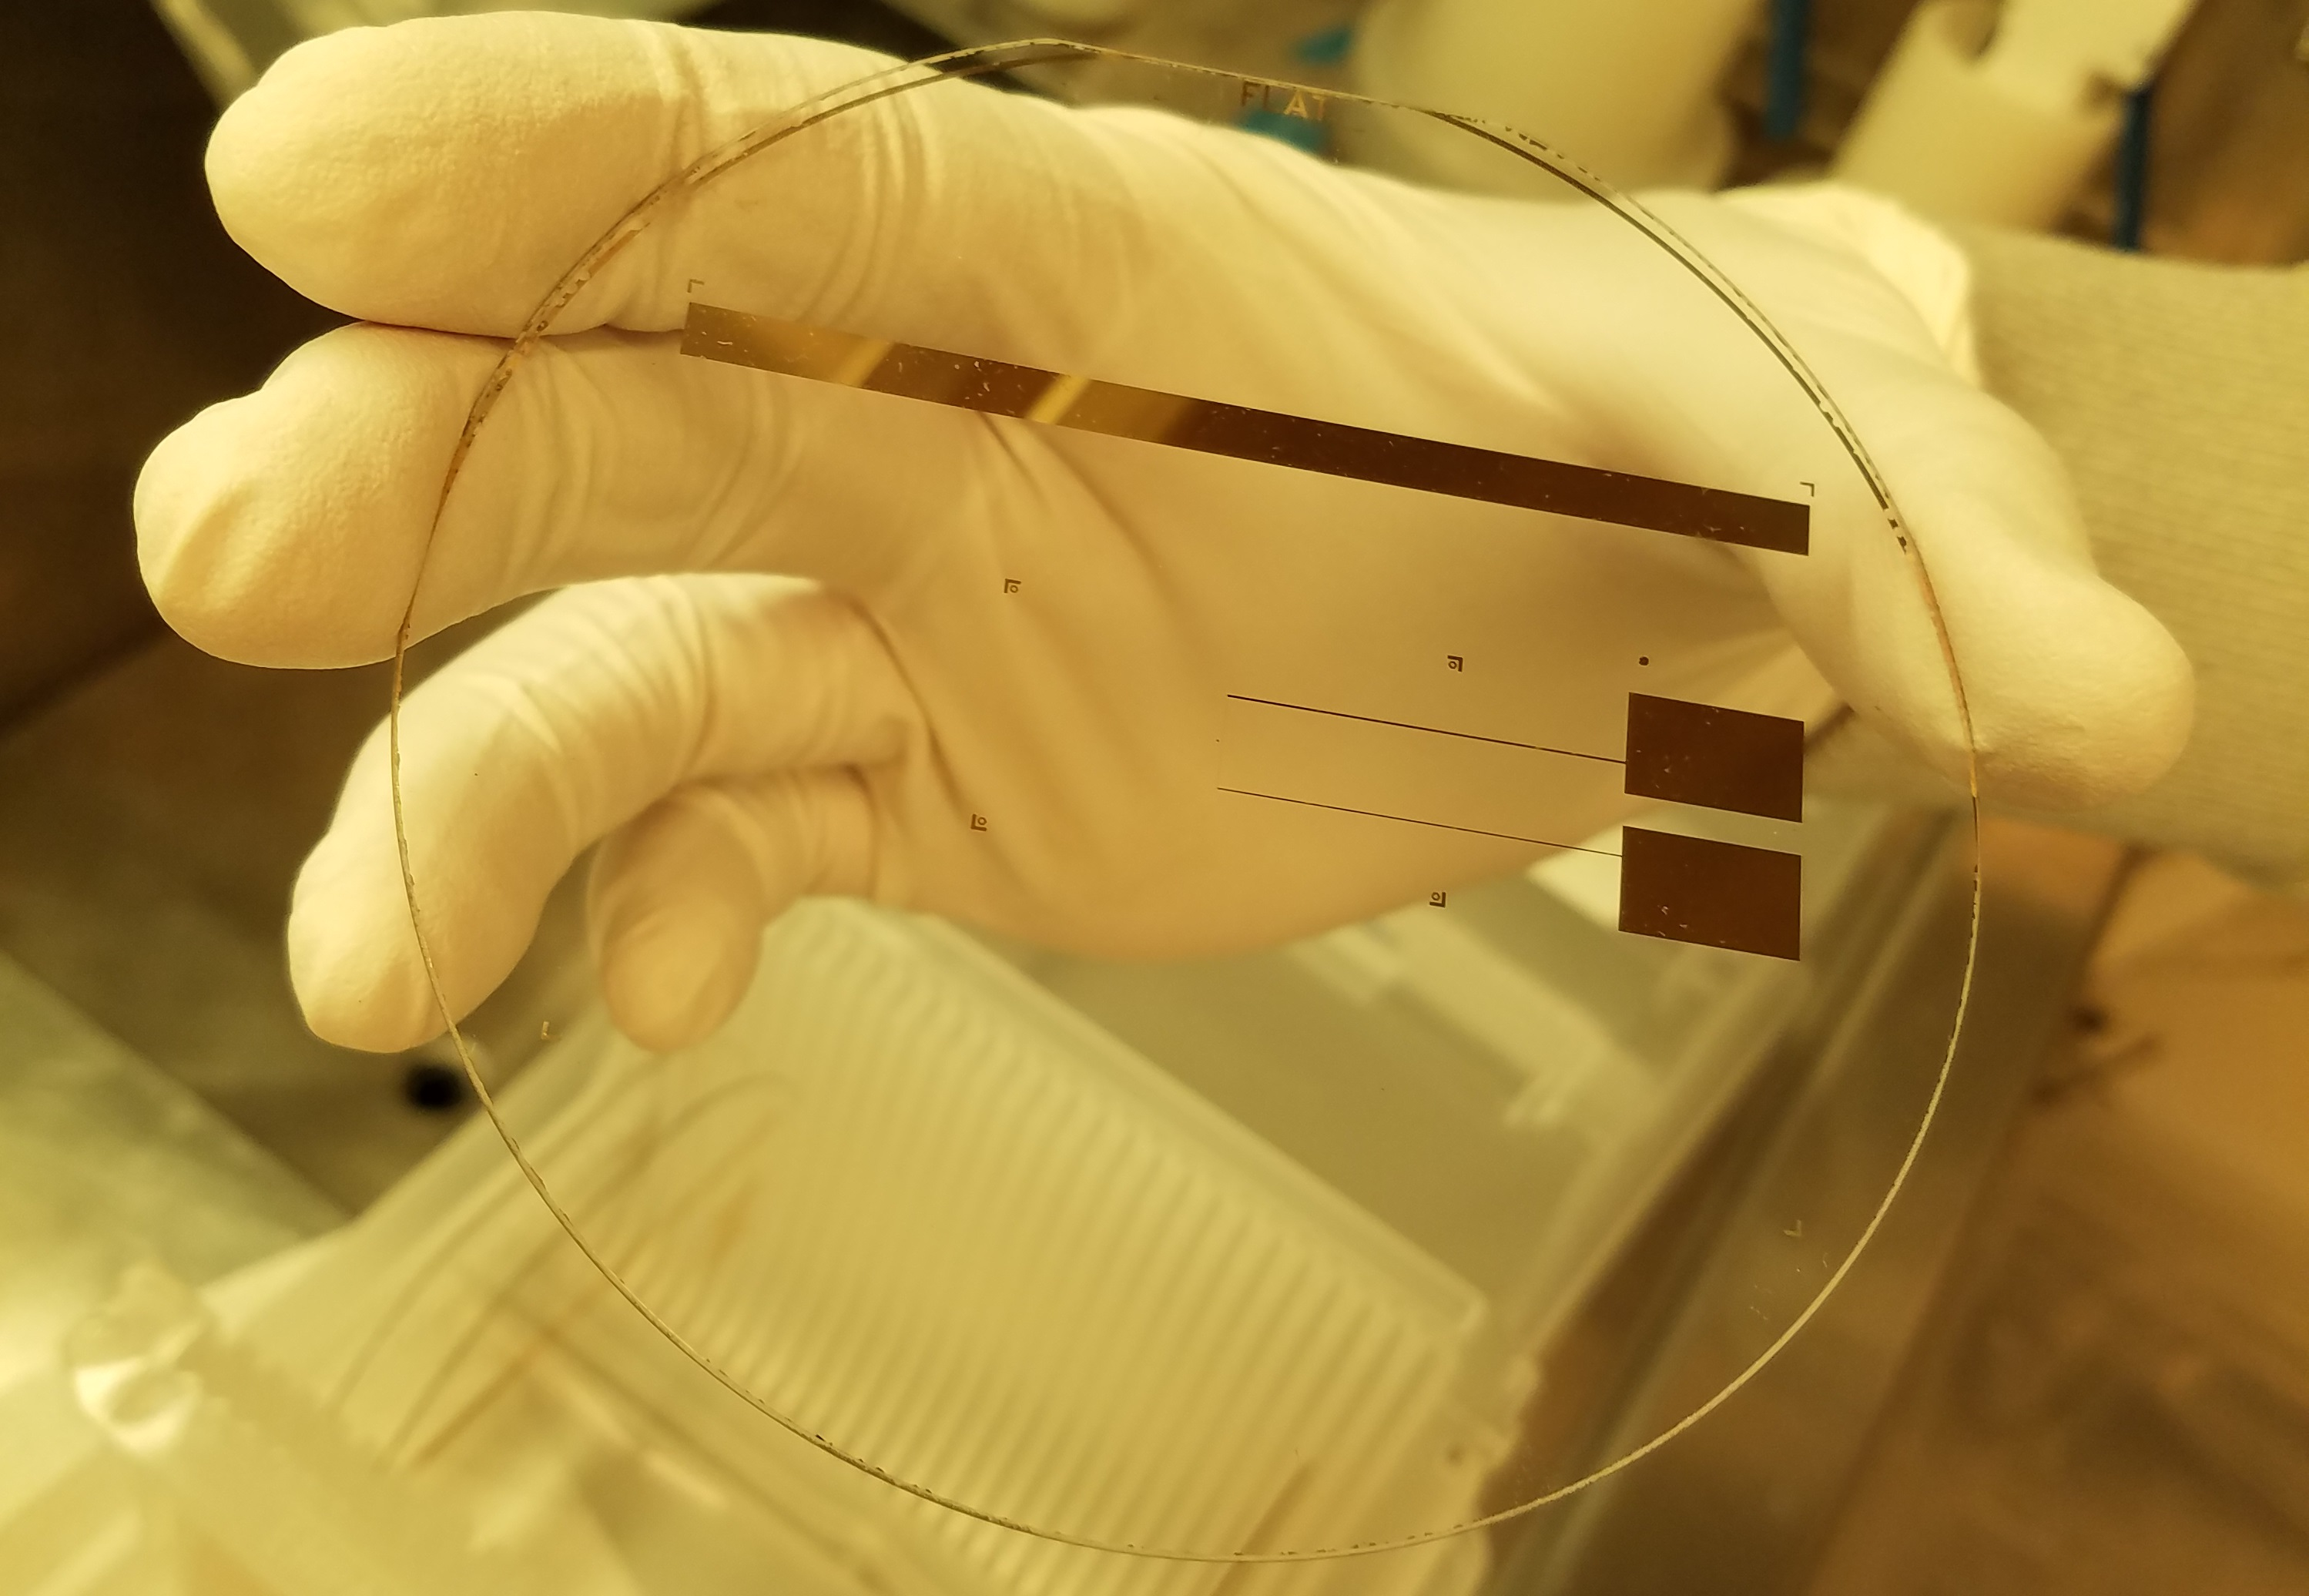
\includegraphics[width=\textwidth]{images/electrodes_real.jpg}
        \caption{Successful fabrication of device electrodes}
    \end{subfigure}
    \\
    \vspace{0.1 in}
    \centering
    \begin{subfigure}[b]{0.45\textwidth}
        \centering
        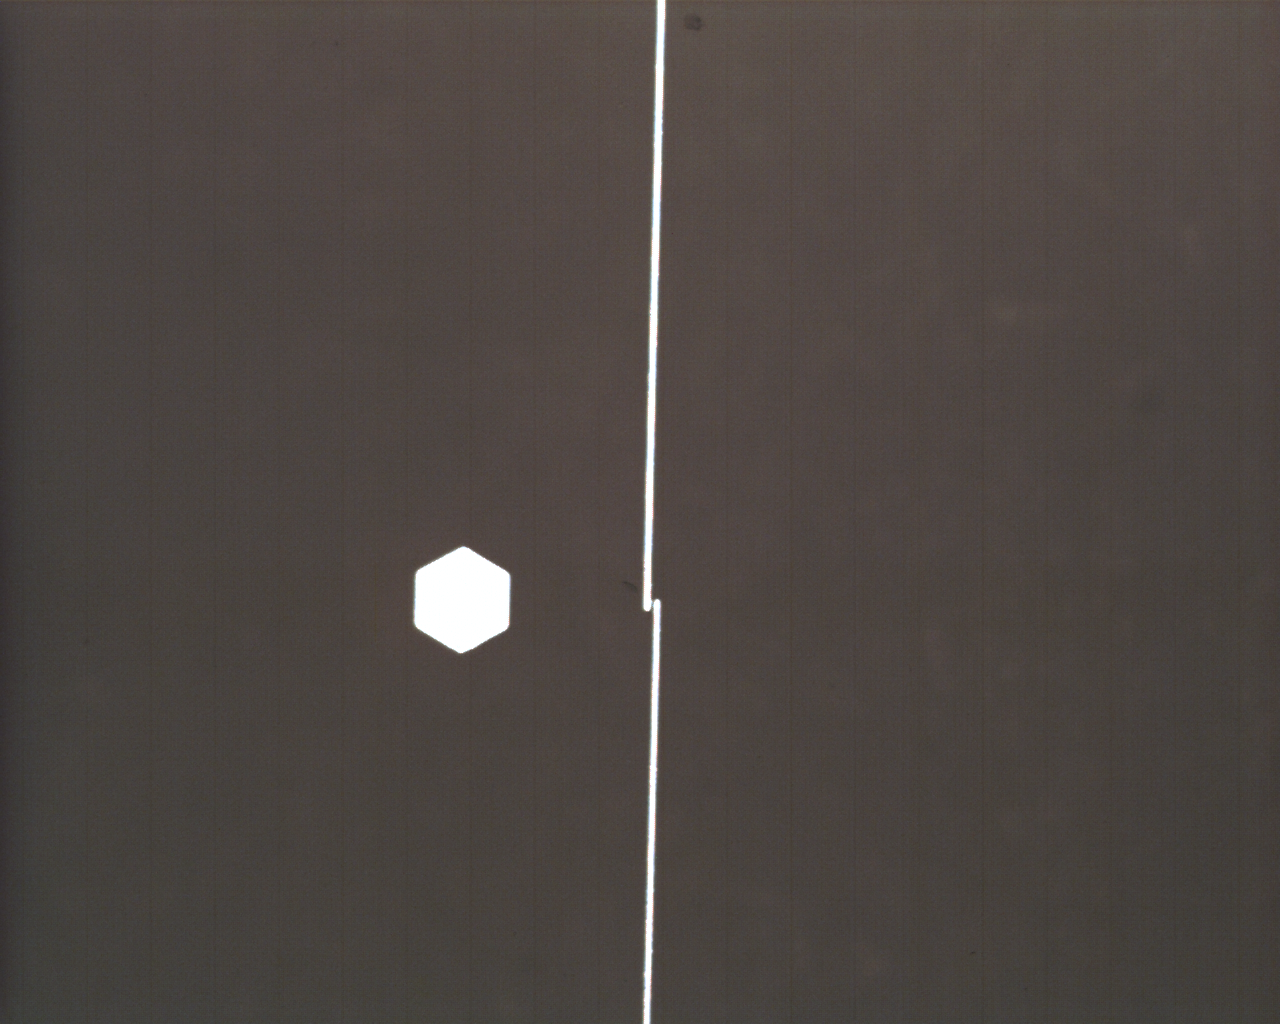
\includegraphics[width=\textwidth]{images/goodElectrode.png}
        \caption{Impedance magnitude and phase}
    \end{subfigure}
    \hfill
    \begin{subfigure}[b]{0.45\textwidth}
        \centering
        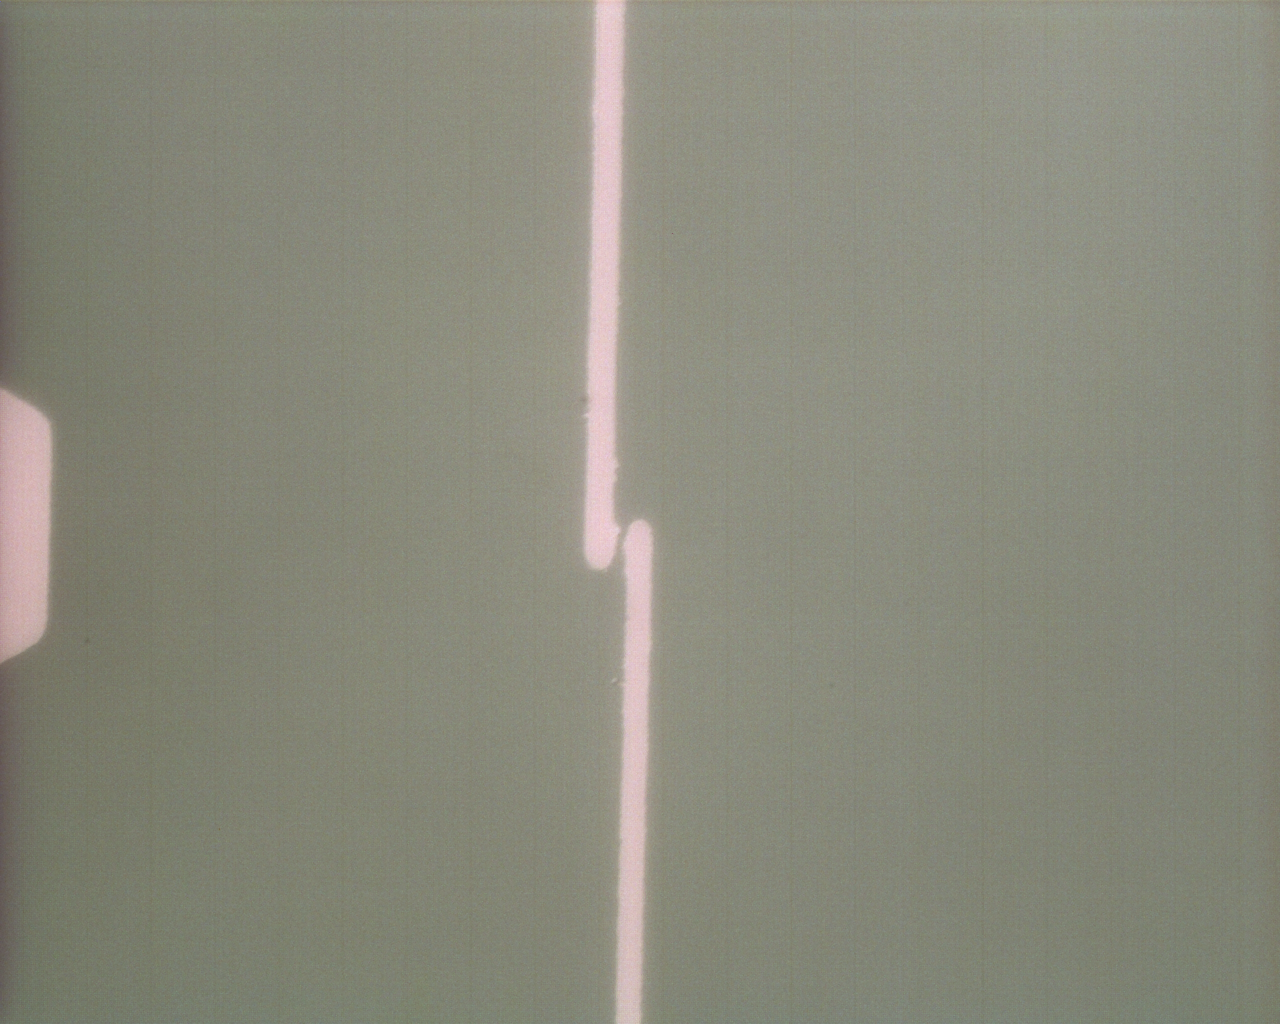
\includegraphics[width=\textwidth]{images/goodElectrodeCloseUp.png}
        \caption{Real and imaginary impedance}
    \end{subfigure}
\end{figure}


\FloatBarrier

\subsection{Device Bonding}


\begin{figure}[h]
    \centering
    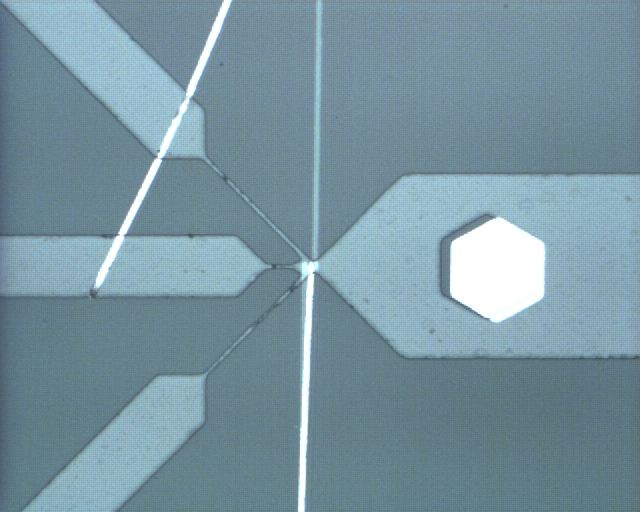
\includegraphics[width=\textwidth]{images/bad_device.png}
    \caption{Failed device}
    \label{fig:bad_device}
\end{figure}


\begin{figure}[h]
    \centering
    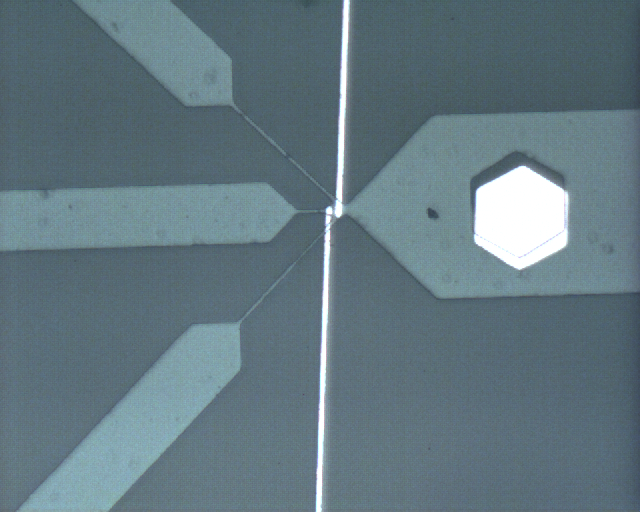
\includegraphics[width=\textwidth]{images/good_device.png}
    \caption{Good device}
    \label{fig:good_device}
\end{figure}

\FloatBarrier

\section{Impedance Spectroscopy System}

\begin{figure}[h]
    \centering
    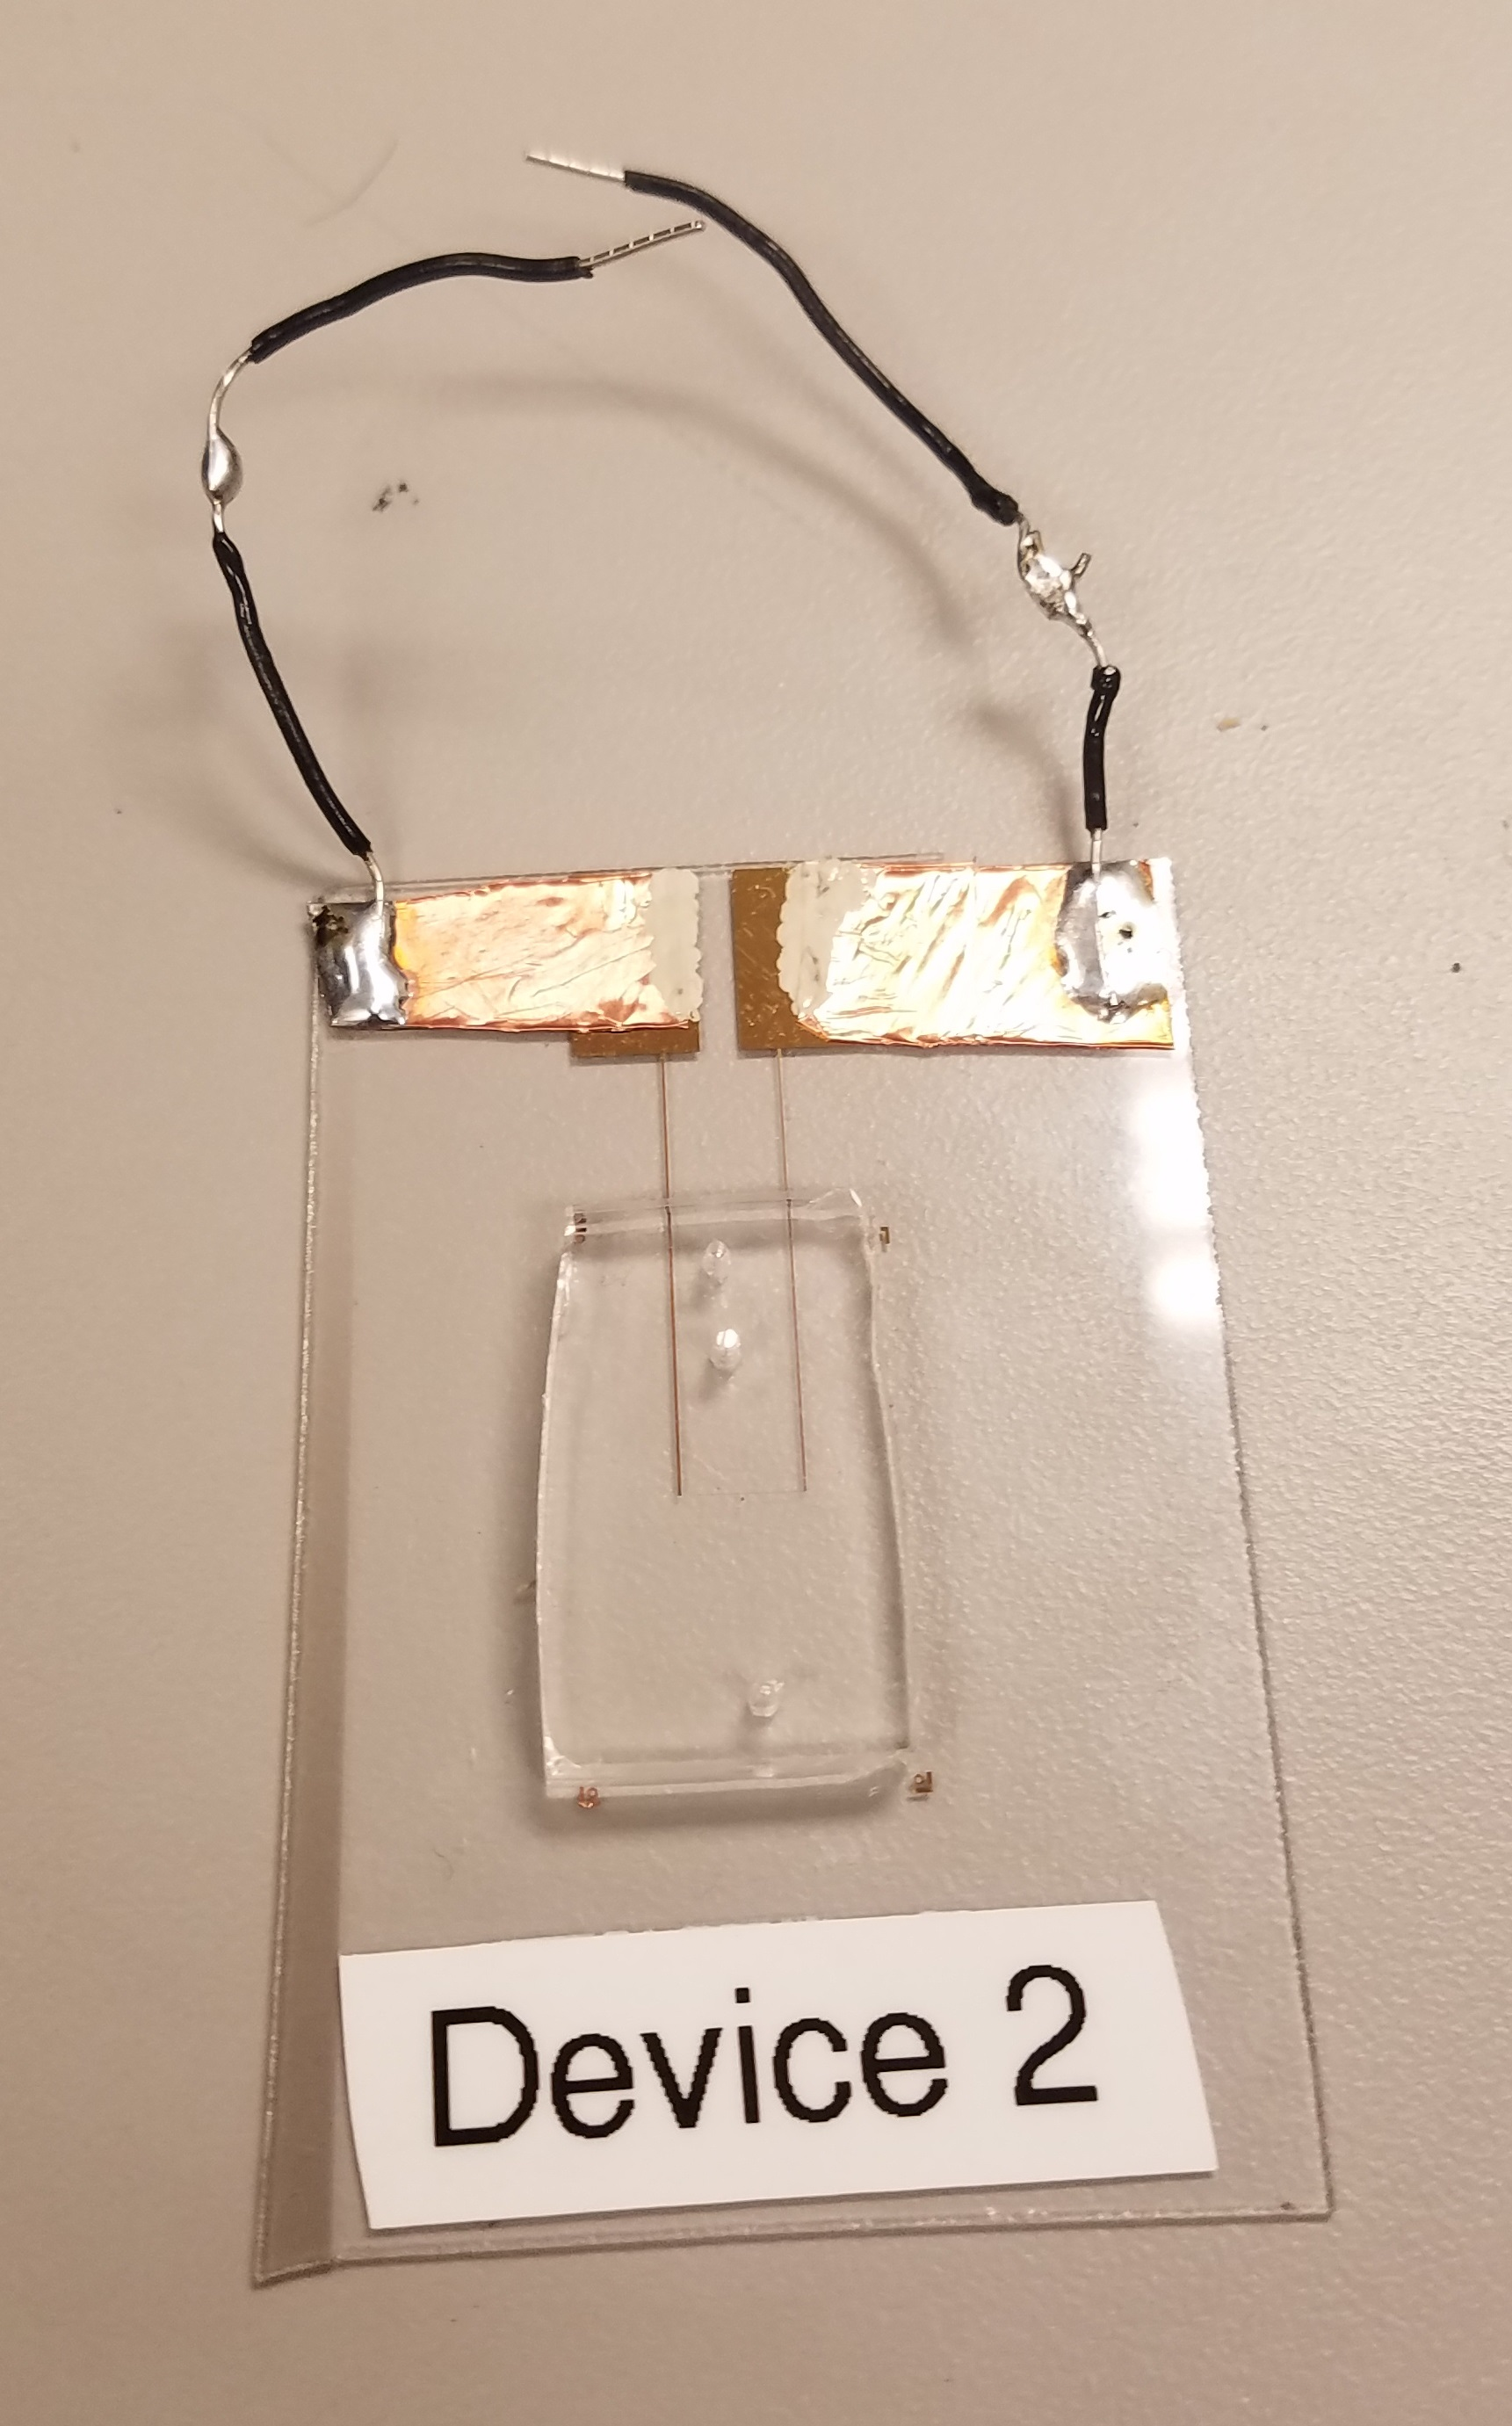
\includegraphics[width=0.5\textwidth]{images/device_22.jpg}
    \caption{Device two}
    \label{fig:my_label}
\end{figure}

\begin{figure}[h]
    \centering
    \begin{subfigure}[b]{0.45\textwidth}
        \centering
        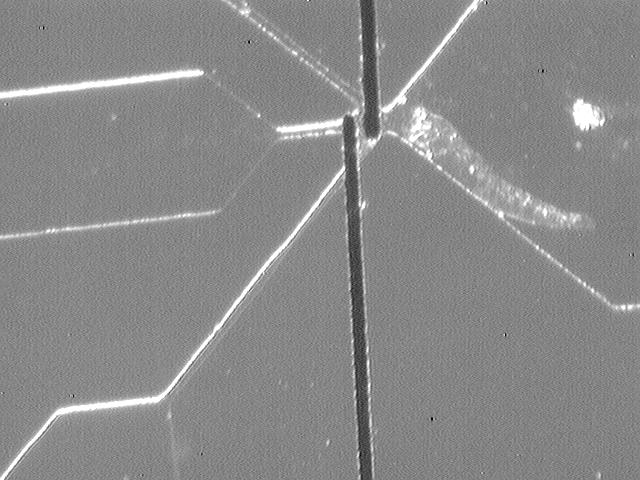
\includegraphics[width=\textwidth]{images/IS_empty.jpg}
        \caption{Sensor chamber fluid filled}
    \end{subfigure}
    \hfill
    \begin{subfigure}[b]{0.45\textwidth}
        \centering
        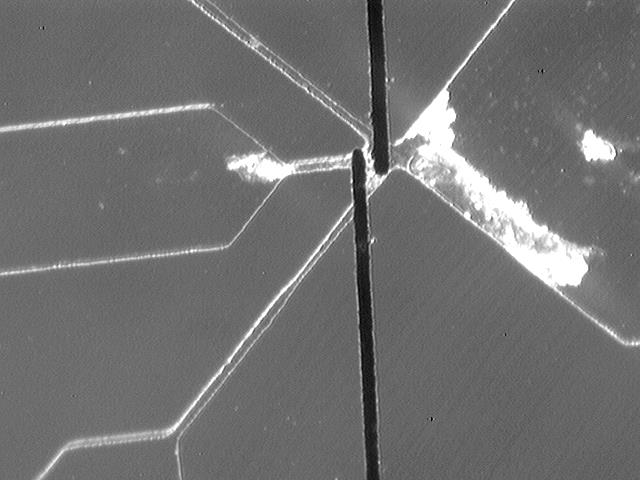
\includegraphics[width=\textwidth]{images/IS_particle_saturation.jpg}
        \caption{Sensor chamber 7$\mu$m }
    \end{subfigure}
    \\
    \vspace{0.1 in}
    \begin{subfigure}[b]{0.45\textwidth}
        \centering
        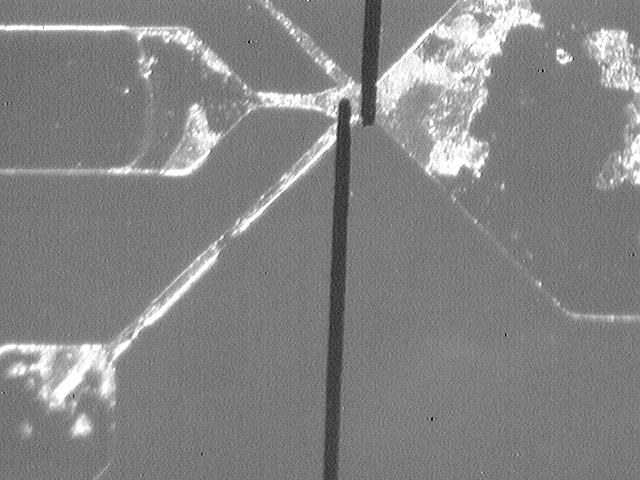
\includegraphics[width=\textwidth]{images/IS_jammed.jpg}
        \caption{Jammed}
    \end{subfigure}
    \hfill
    \begin{subfigure}[b]{0.45\textwidth}
        \centering
        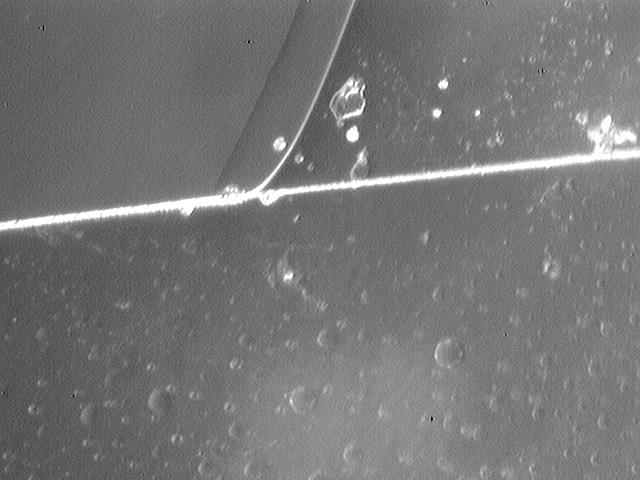
\includegraphics[width=\textwidth]{images/IS_device_delamination.jpg}
        \caption{Device delamination}
    \end{subfigure}
    \caption{IS device sensor region images.}
    \label{fig:IS_sensor_reigon_measurement}
\end{figure}

\begin{figure}[h]
    \centering
    \begin{subfigure}[b]{\textwidth}
        \centering
        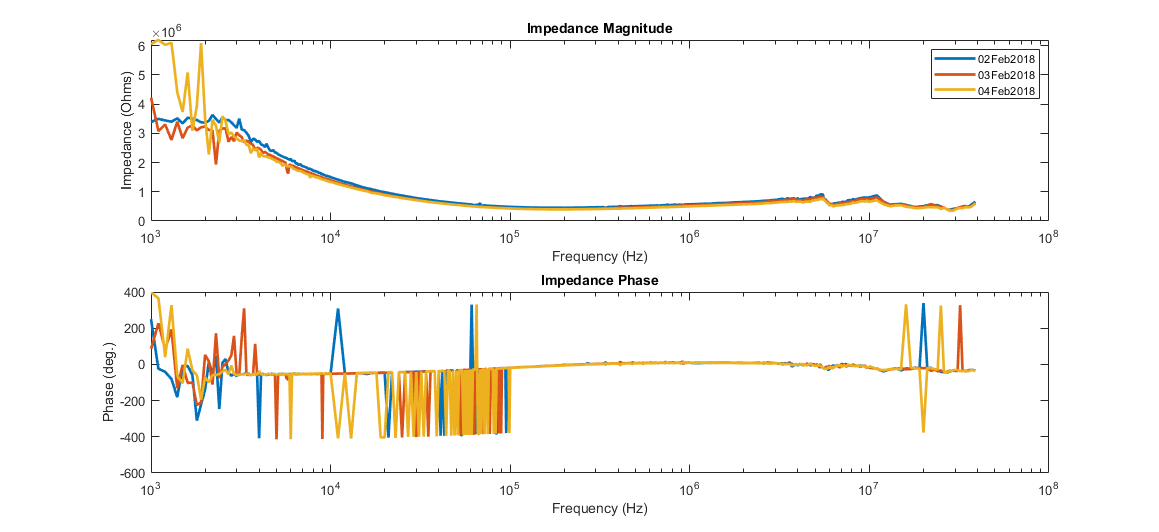
\includegraphics[width=\textwidth]{images/reproducibility_PBS_mag_phase.png}
        \caption{Sensor chamber fluid filled}
    \end{subfigure}
    \\
    \vspace{0.1 in}
    \begin{subfigure}[b]{\textwidth}
        \centering
        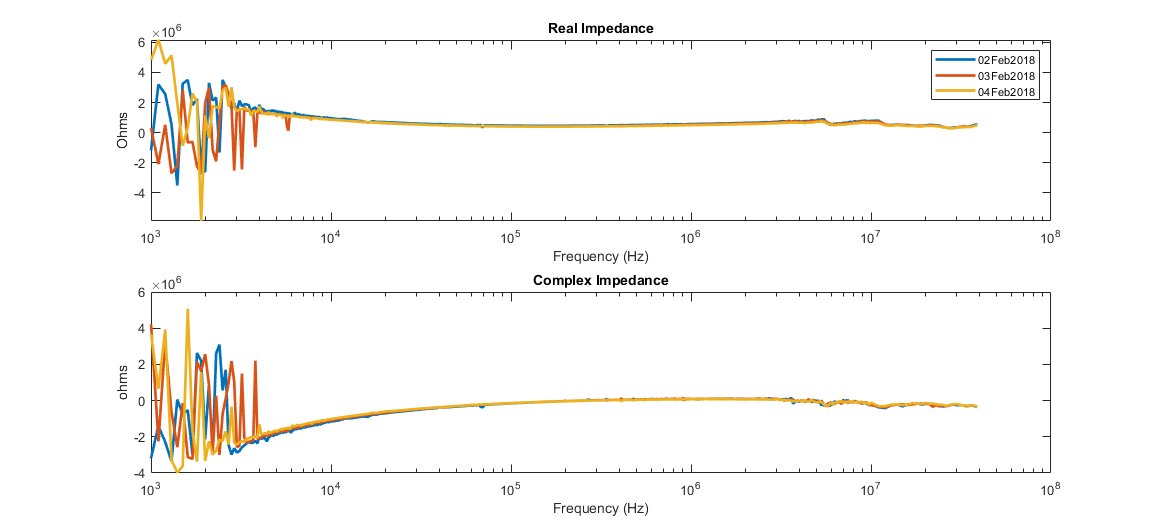
\includegraphics[width=\textwidth]{images/reproducibility_PBS_real_imag.png}
        \caption{Sensor chamber 7$\mu$m }
    \end{subfigure}
    \caption{Impedance spectroscopy reproducibility demonstrated with repeated measurement of phosphate buffered solution over a span of three days.}
    \label{fig:IS_data_reproducibility}
\end{figure}

\begin{figure}[h]
    \centering
    \begin{subfigure}[b]{\textwidth}
        \centering
        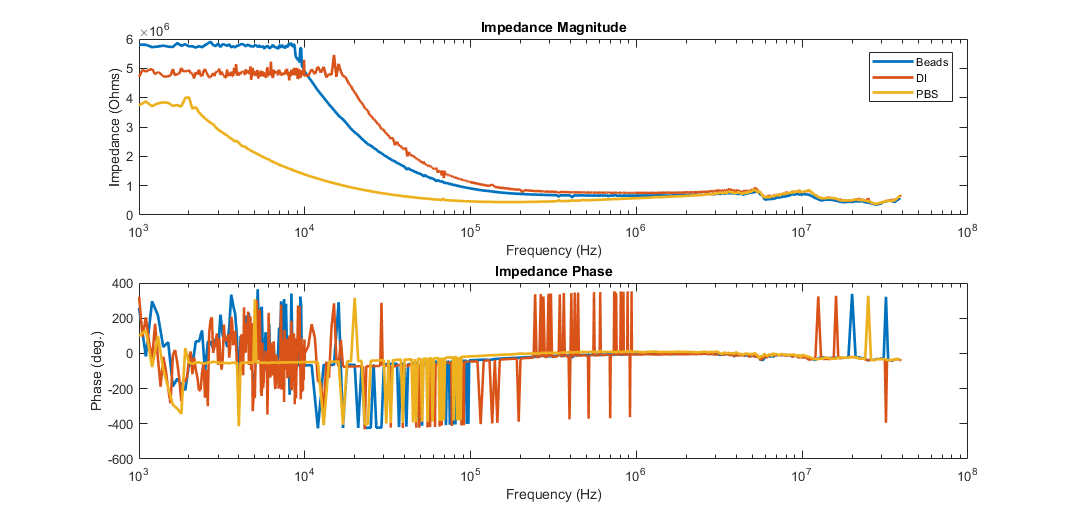
\includegraphics[width=\textwidth]{images/raw_IS_data_mag_phase.png}
        \caption{Sensor chamber fluid filled}
    \end{subfigure}
    \\
    \vspace{0.1 in}
    \begin{subfigure}[b]{\textwidth}
        \centering
        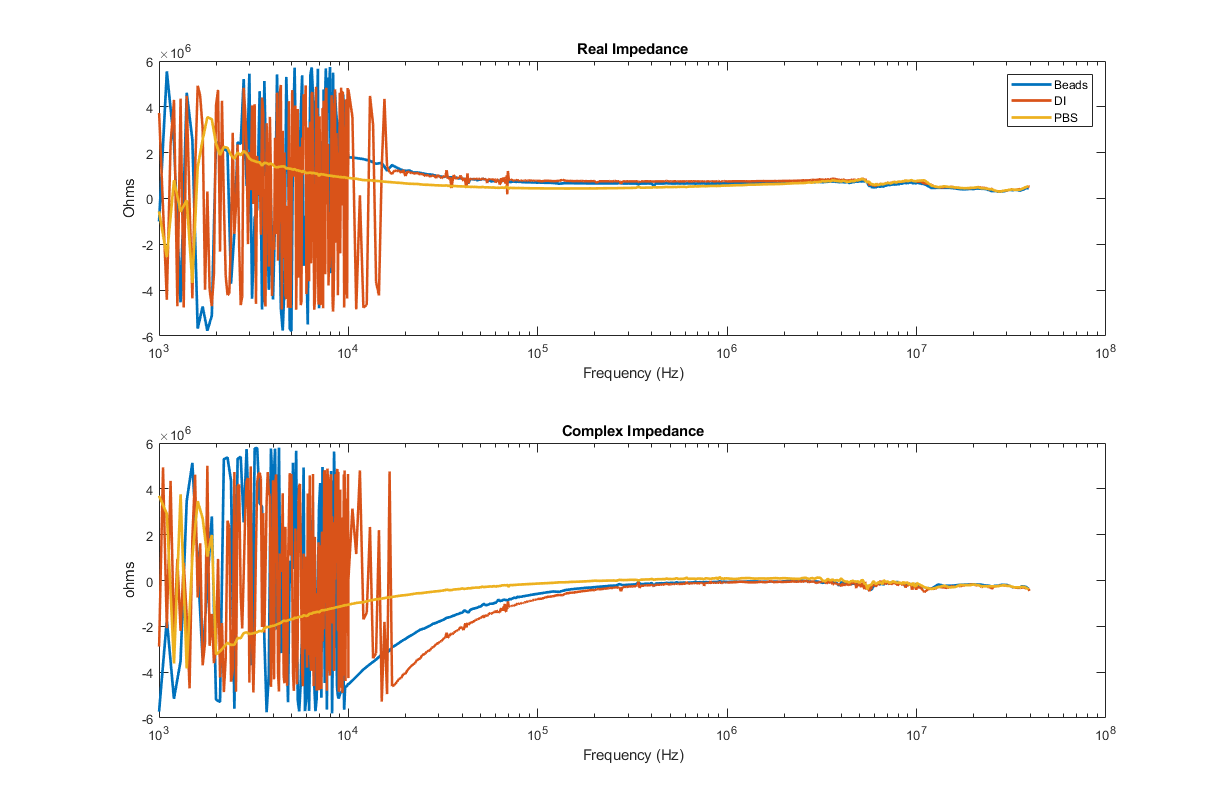
\includegraphics[width=\textwidth]{images/raw_IS_data_real_imag.png}
        \caption{Sensor chamber 7$\mu$m }
    \end{subfigure}
    \\
%    \vspace{0.1 in}
%    \begin{subfigure}[b]{\textwidth}
%        \centering
%        \includegraphics[width=\textwidth]{images/raw_IS_%data_nyquist.png}
%        \caption{Jammed}
%    \end{subfigure}
    \caption[PBS, DI, microbead IS data comparison.]{Comparison of impedance spectroscopy results from measurements of phosphate buffered solution, de-ionized water, and the chamber saturated with 7 $\mu$m polystyrene beads.}
    \label{fig:IS_data_beads_pbs_DI_comp}
\end{figure}

\begin{figure}[h]
    \centering
    \begin{subfigure}[b]{\textwidth}
        \centering
        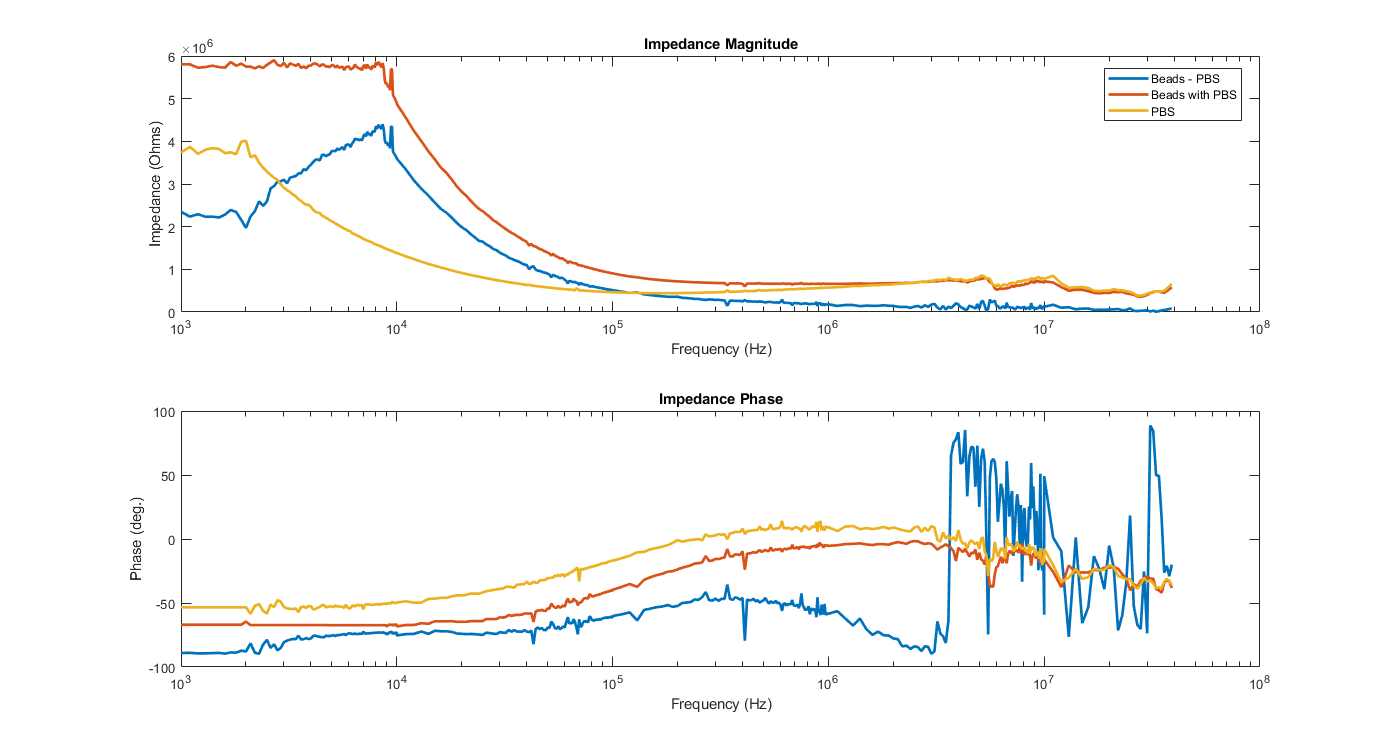
\includegraphics[width=\textwidth]{images/IS_data_clean_mag_phase.png}
        \caption{Sensor chamber fluid filled}
    \end{subfigure}
    \\
    \vspace{0.1 in}
    \begin{subfigure}[b]{\textwidth}
        \centering
        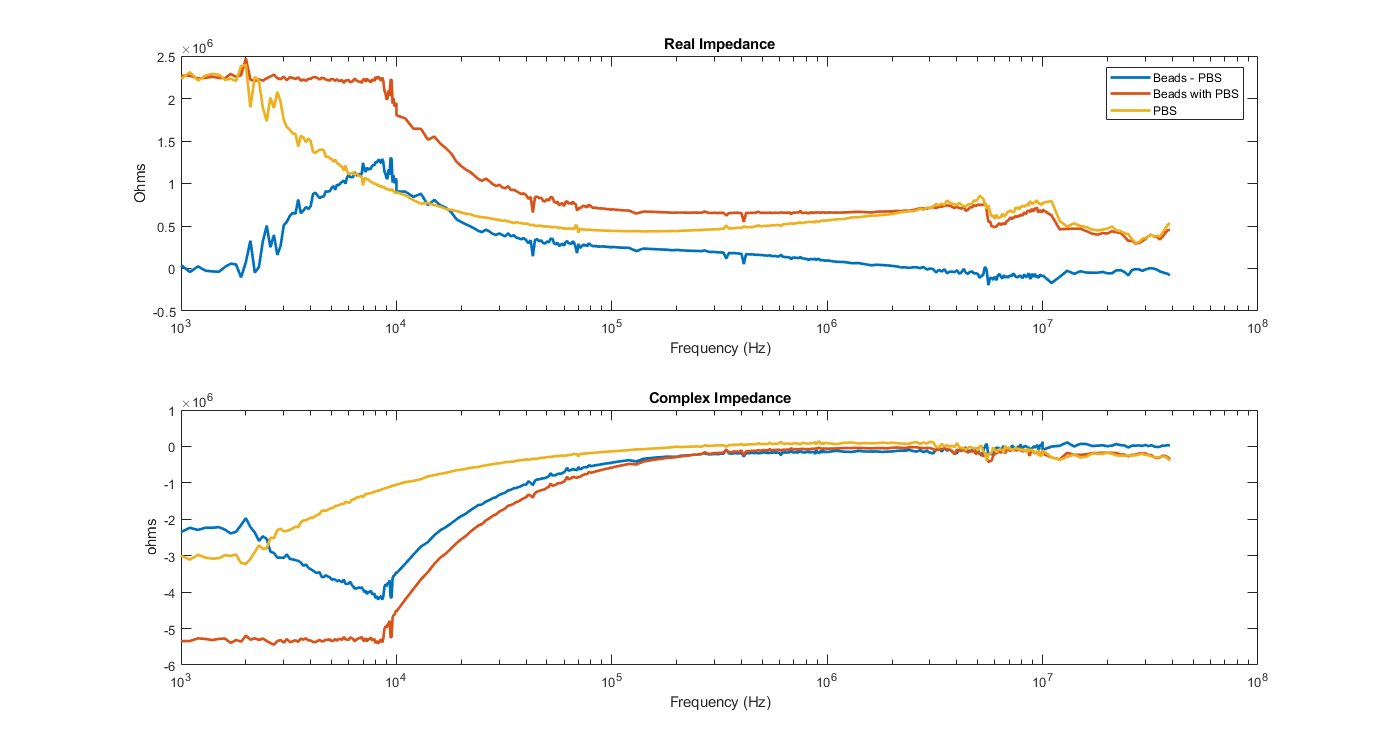
\includegraphics[width=\textwidth]{images/IS_data_clean_real_imag.png}
        \caption{Sensor chamber 7$\mu$m }
    \end{subfigure}
    \\
    \vspace{0.1 in}
    \begin{subfigure}[b]{\textwidth}
        \centering
        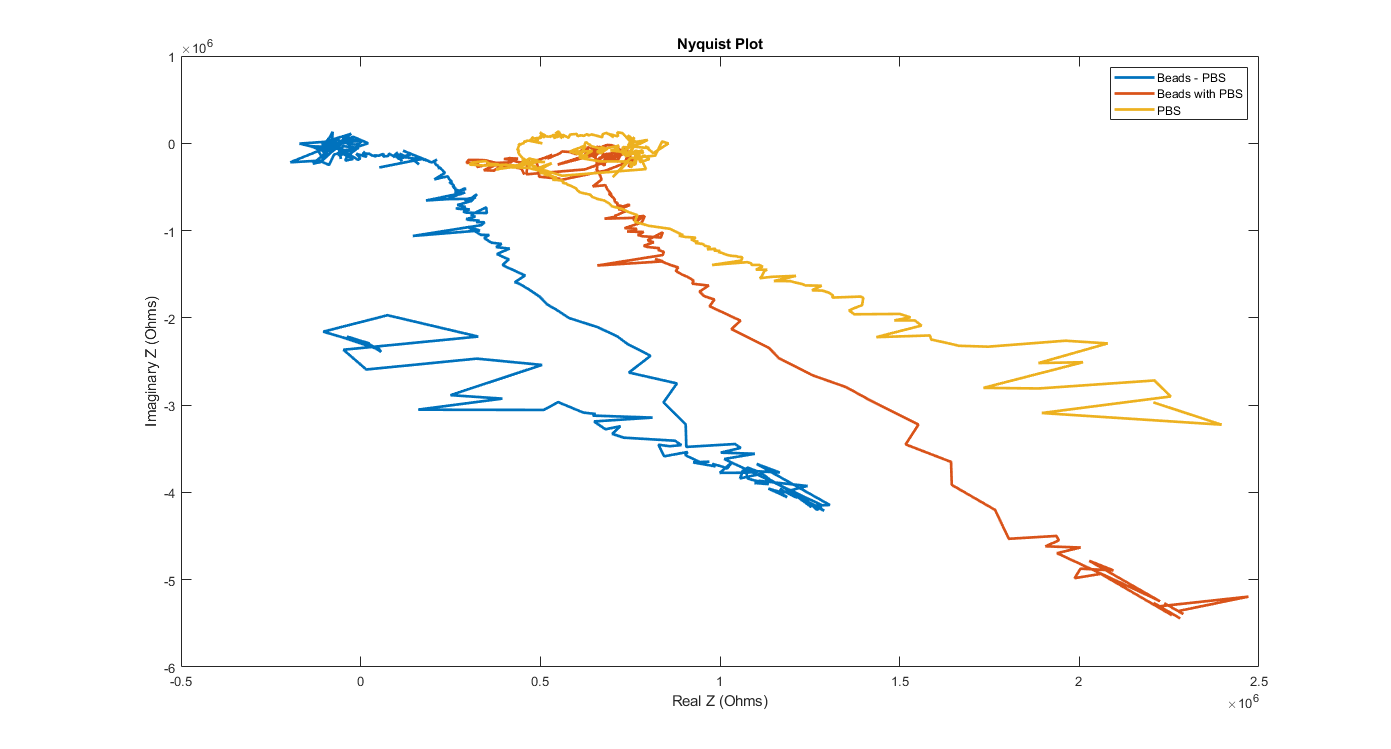
\includegraphics[width=\textwidth]{images/IS_data_clean_nyquist.png}
        \caption{Jammed}
    \end{subfigure}
    \caption[PBS, PBS saturated with micro-beads, and the phasor difference.]{Comparison of impedance spectroscopy results from measurements of phosphate buffered solution, phosphate buffered solution saturated with 7 $\mu$m polystyrene beads, and the phasor difference between the two. The phase data was cleaned and the real and imaginary impedance was re-calculated.}
    \label{fig:IS_data_pbs_pbsBeads_difference}
\end{figure}

\begin{figure}[h]
    \centering
    \begin{subfigure}[b]{\textwidth}
        \centering
        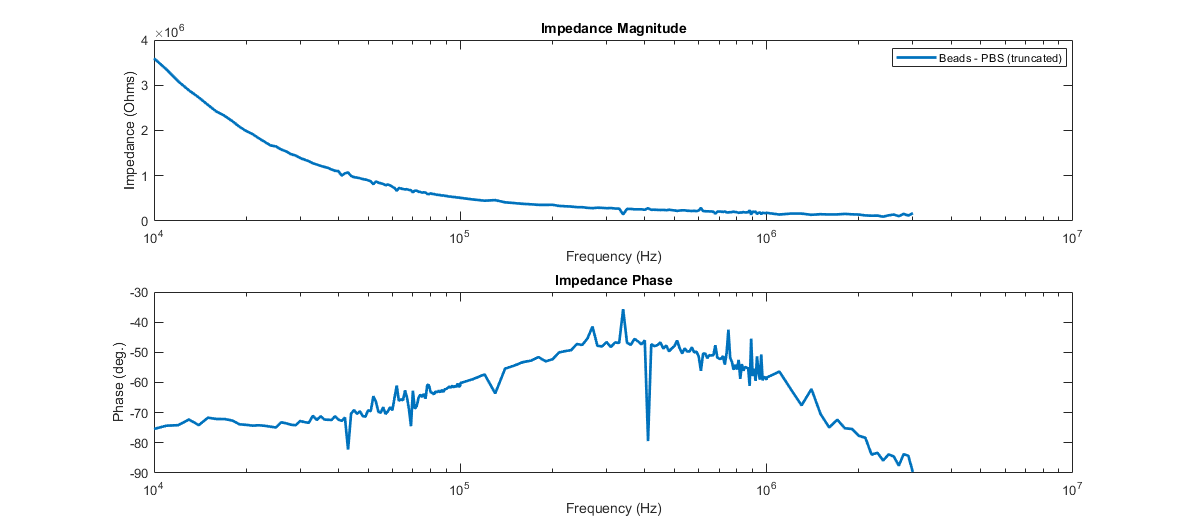
\includegraphics[width=\textwidth]{images/IS_data_beads-PBS_truncated_mag_phase.png}
        \caption{Sensor chamber fluid filled}
    \end{subfigure}
    \\
    \vspace{0.1 in}
    \begin{subfigure}[b]{\textwidth}
        \centering
        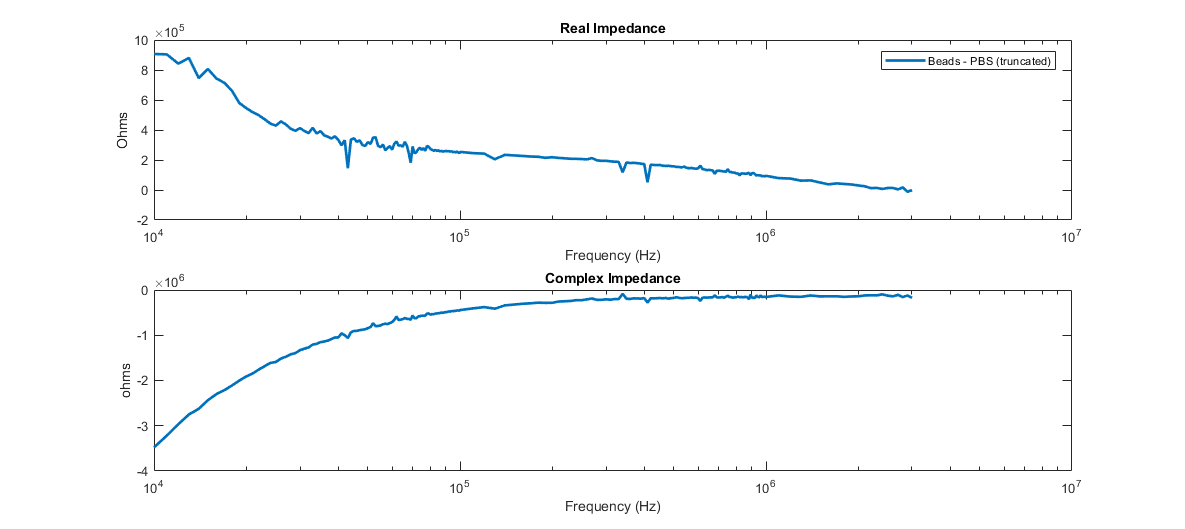
\includegraphics[width=\textwidth]{images/IS_data_beads-PBS_truncated_real_imag.png}
        \caption{Sensor chamber 7$\mu$m }
    \end{subfigure}
    \\
    \vspace{0.1 in}
    \begin{subfigure}[b]{\textwidth}
        \centering
        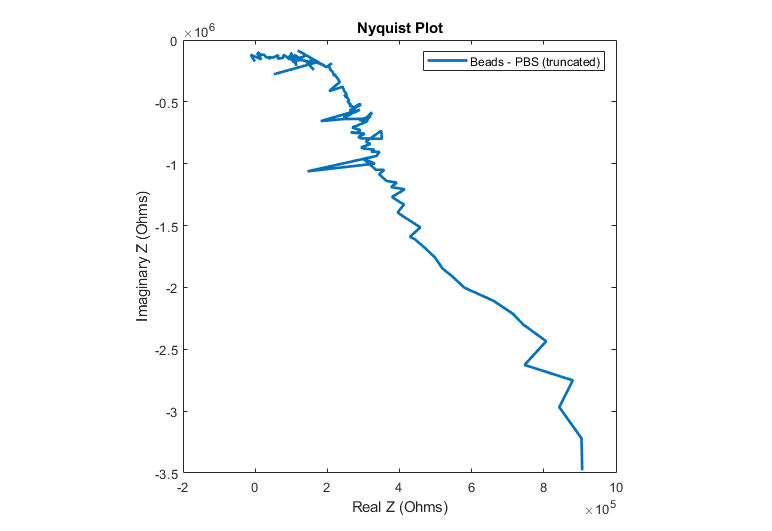
\includegraphics[width=\textwidth]{images/IS_data_beads-PBS_nyquist.png}
        \caption{Jammed}
    \end{subfigure}
    \caption[Truncated phasor difference between PBS, and micro-bead saturated PBS.]{Phasor difference between the PBS solution, and PBS solution saturated with 7$\mu$m microbeads. The data was truncated to the reliable frequency range of $10^4$ to $3x10^6$ hz.}
    \label{fig:IS_data_beads_pbs_DI_comp}
\end{figure}


\FloatBarrier

\section{Modeling}

\subsection{Impedance Spectroscopy Results}

\begin{figure}[h]
    \centering
    \begin{subfigure}[b]{\textwidth}
        \centering
        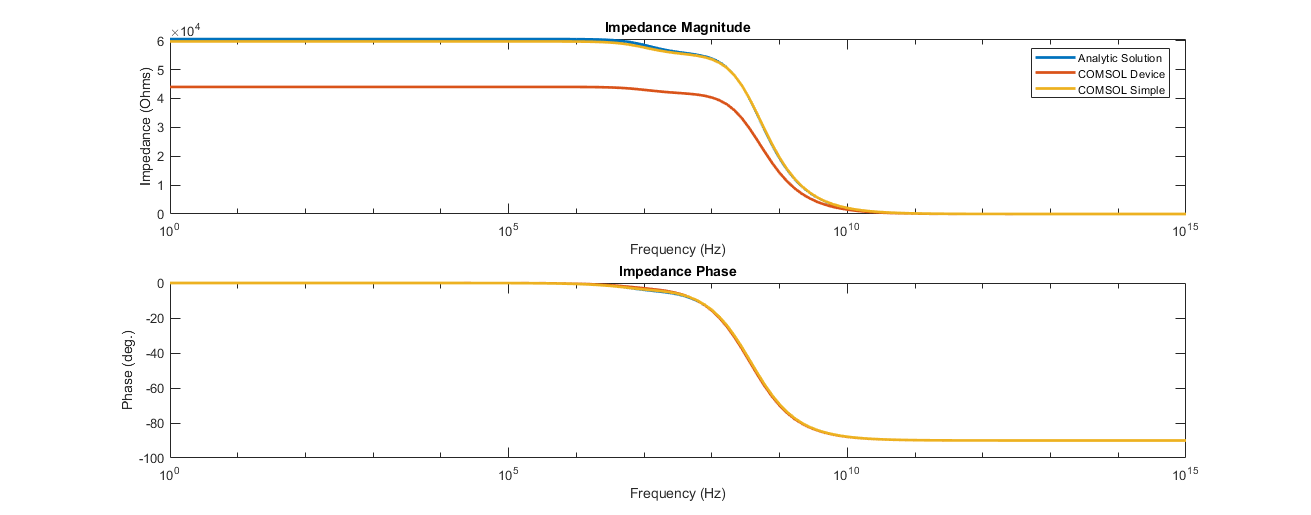
\includegraphics[width=\textwidth]{images/IS_model_mag_phase.png}
        \caption{Sensor chamber fluid filled}
    \end{subfigure}
    \\
    \vspace{0.1 in}
    \begin{subfigure}[b]{\textwidth}
        \centering
        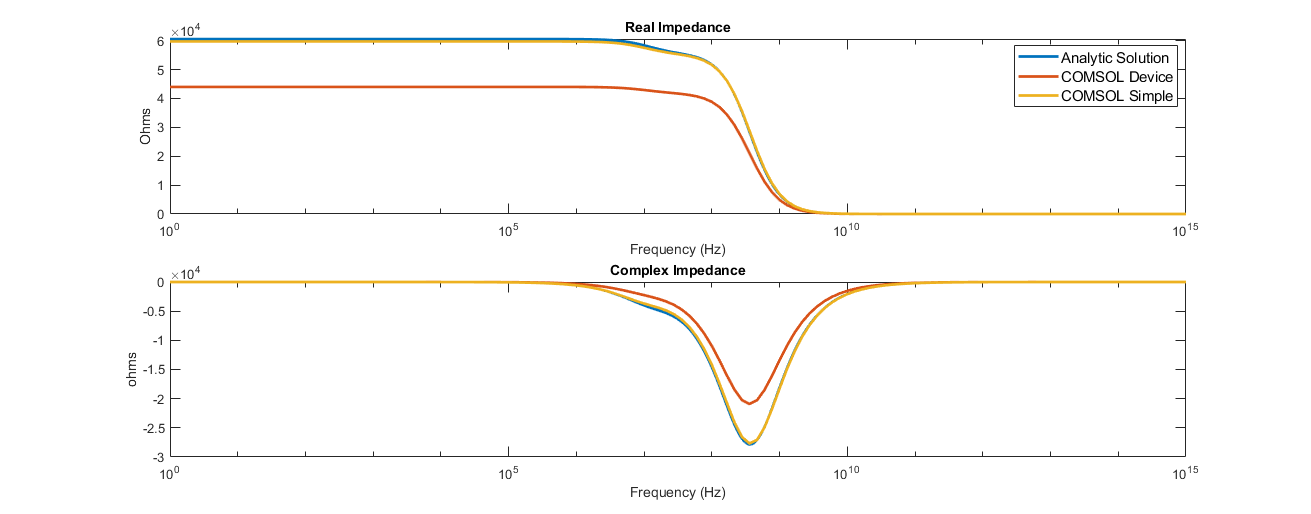
\includegraphics[width=\textwidth]{images/IS_model_real_imag.png}
        \caption{Sensor chamber 7$\mu$m }
    \end{subfigure}
    \\
    \vspace{0.1 in}
    \begin{subfigure}[b]{\textwidth}
        \centering
        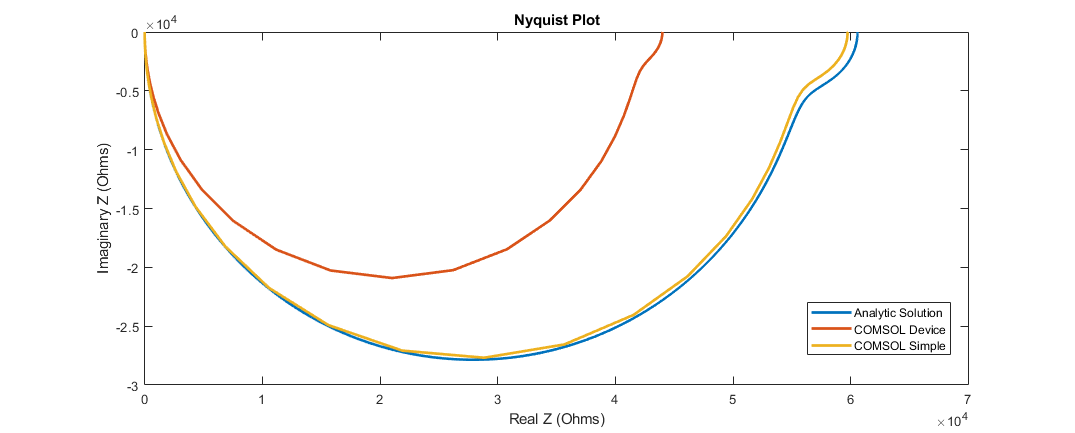
\includegraphics[width=\textwidth]{images/IS_model_nyquist.png}
        \caption{Jammed}
    \end{subfigure}
    \caption[Analyitic and FEA generated single cell impedance spectrums]{Single cell impedance spectrum generated by the analytic impedance solution, the simple FEA model, and the device FEA model.}
    \label{fig:single_cell_model_IS_data}
\end{figure}

\begin{figure}[h]
    \centering
    \begin{subfigure}[b]{\textwidth}
        \centering
        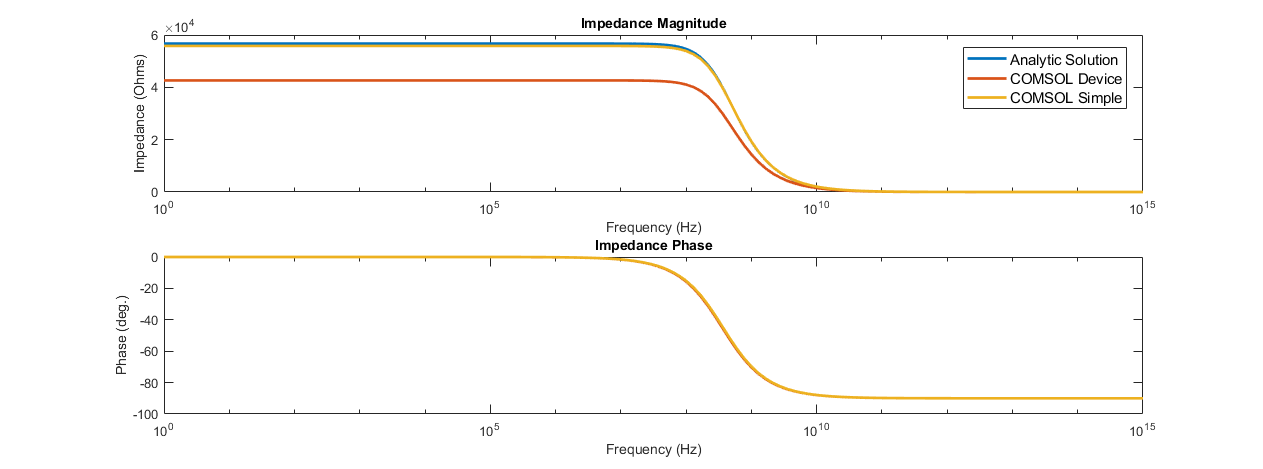
\includegraphics[width=\textwidth]{images/IS_model_medium_mag_phase.png}
        \caption{Sensor chamber fluid filled}
    \end{subfigure}
    \\
    \vspace{0.1 in}
    \begin{subfigure}[b]{\textwidth}
        \centering
        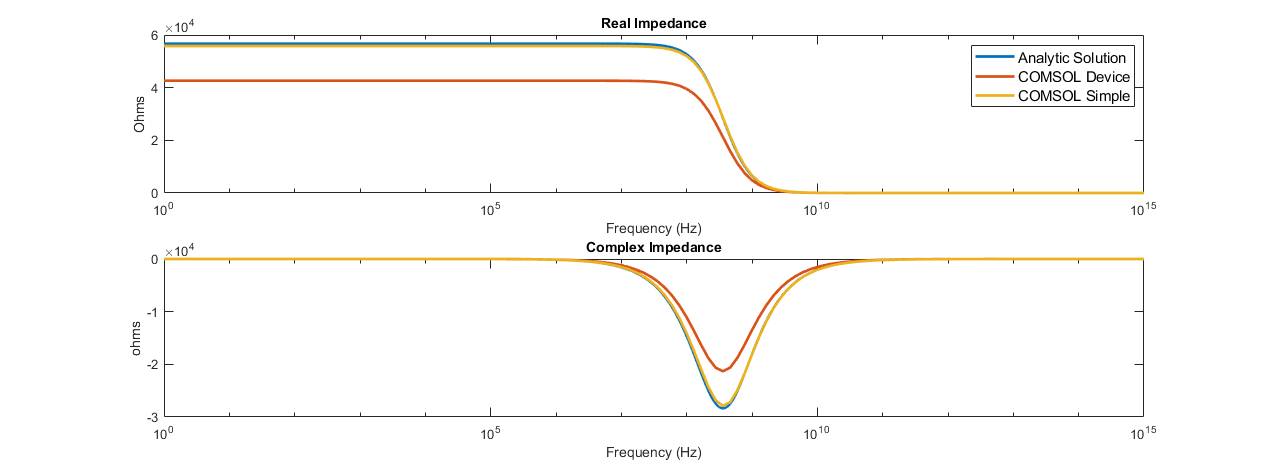
\includegraphics[width=\textwidth]{images/IS_model_medium_real_imag.png}
        \caption{Sensor chamber 7$\mu$m }
    \end{subfigure}
    \\
    \vspace{0.1 in}
    \begin{subfigure}[b]{\textwidth}
        \centering
        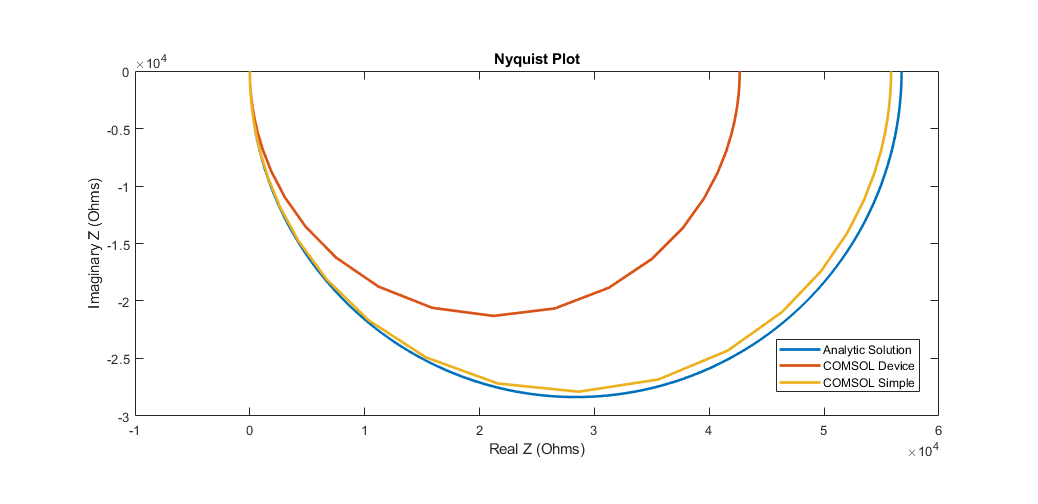
\includegraphics[width=\textwidth]{images/IS_model_medium_nyquist.png}
        \caption{Jammed}
    \end{subfigure}
    \caption[Analyitic and FEA generated medium impedance spectrum]{Medium impedance spectrum generated by the analytic impedance solution, the simple FEA model, and the device FEA model.}
    \label{fig:medium_model_IS_data}
\end{figure}

\begin{figure}[h]
    \centering
    \begin{subfigure}[b]{\textwidth}
        \centering
        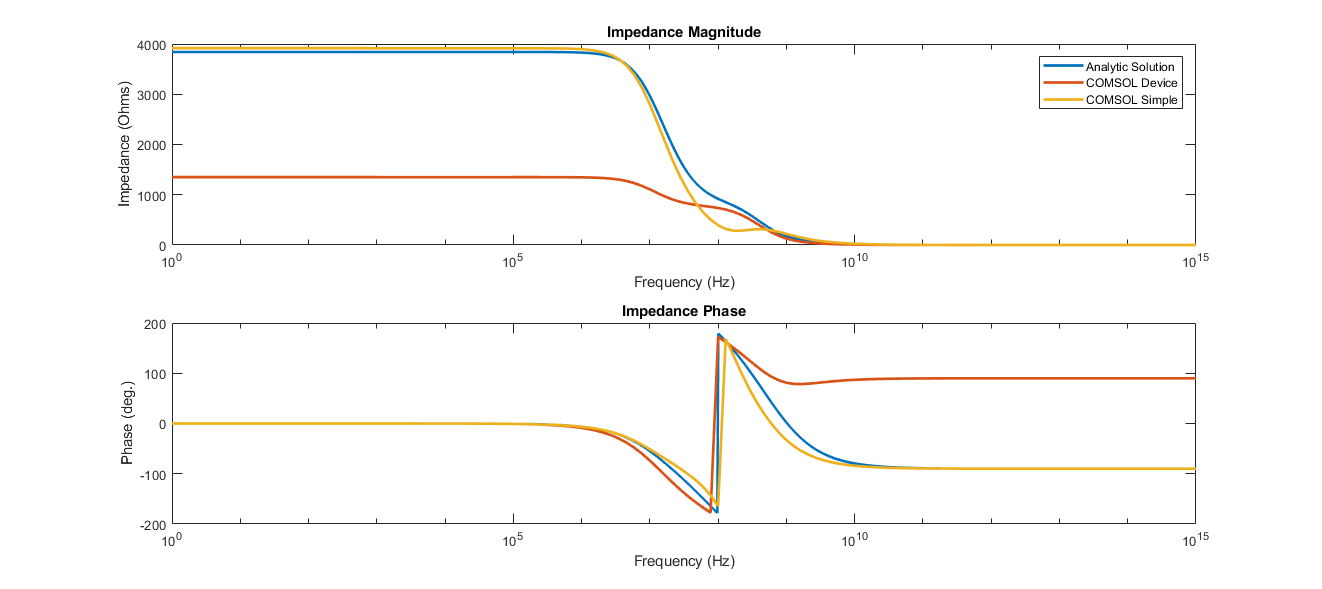
\includegraphics[width=\textwidth]{images/IS_model_difference_mag_phase.png}
        \caption{Sensor chamber fluid filled}
    \end{subfigure}
    \\
    \vspace{0.1 in}
    \begin{subfigure}[b]{\textwidth}
        \centering
        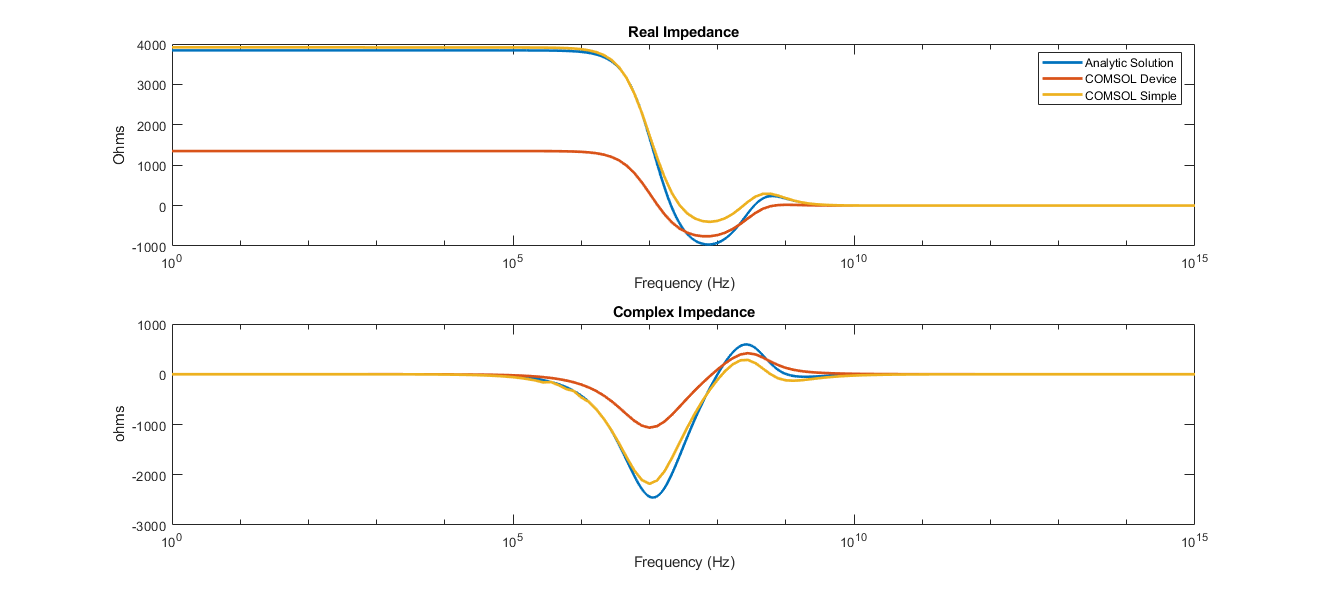
\includegraphics[width=\textwidth]{images/IS_model_difference_real_imag.png}
        \caption{Sensor chamber 7$\mu$m }
    \end{subfigure}
    \\
    \vspace{0.1 in}
    \begin{subfigure}[b]{\textwidth}
        \centering
        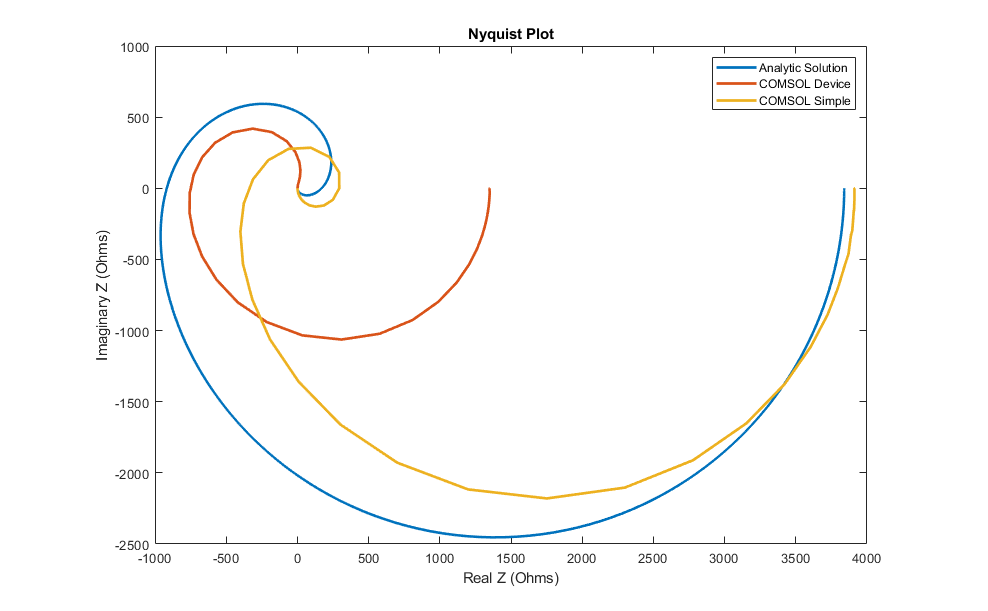
\includegraphics[width=\textwidth]{images/IS_model_difference_nyquist.png}
        \caption{Jammed}
    \end{subfigure}
    \caption[Phasor difference between model mixture and medium impedance spectrum.]{Phasor difference between model mixture and medium impedance spectrum.}
    \label{fig:single_cell_model_IS_data}
\end{figure}

\begin{figure}[h]
    \centering
    \begin{subfigure}[b]{\textwidth}
        \centering
        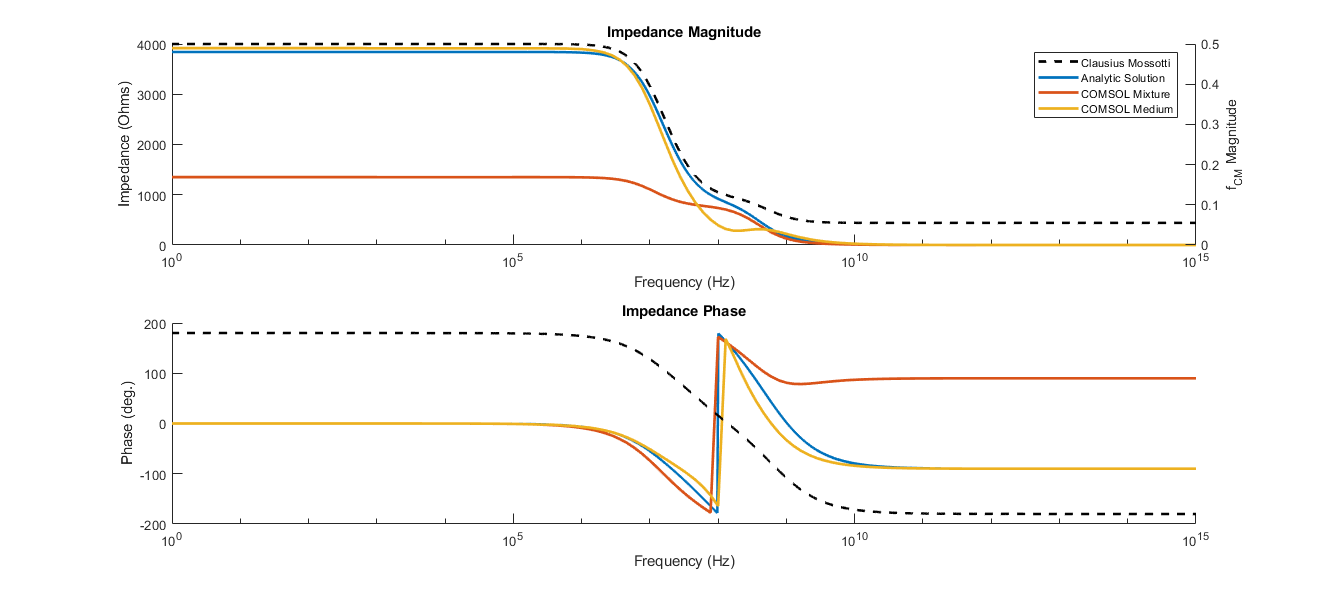
\includegraphics[width=\textwidth]{images/IS_model_difference_mag_phase_CM_overlay.png}
        \caption{Sensor chamber fluid filled}
    \end{subfigure}
    \\
    \vspace{0.1 in}
    \begin{subfigure}[b]{\textwidth}
        \centering
        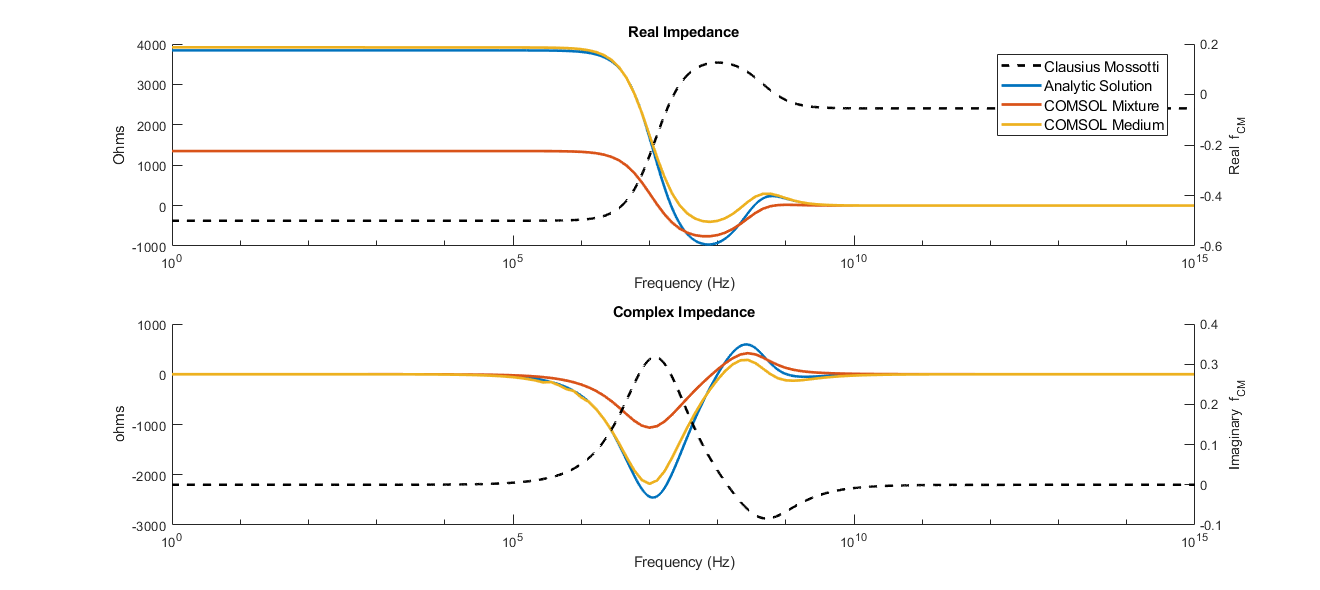
\includegraphics[width=\textwidth]{images/IS_model_real_imag_difference_CM_overlay.png}
        \caption{Sensor chamber 7$\mu$m }
    \end{subfigure}

    \caption[Clausius Mossotti factor overlay on IS model data.]{Clausius Mossotti factor overlay on IS model data.}
    \label{fig:IS_model_difference_fcm_overlay}
\end{figure}

\begin{figure}[h]
    \centering
    \begin{subfigure}[b]{\textwidth}
        \centering
        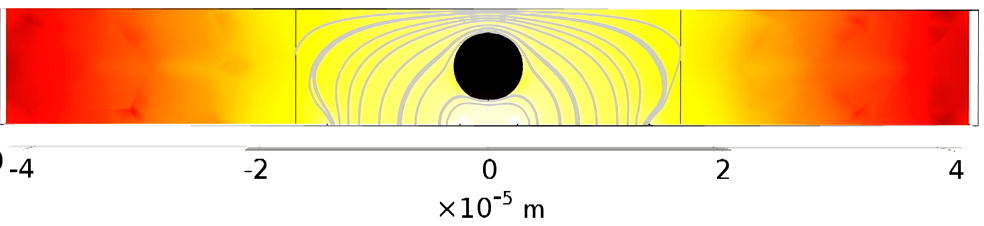
\includegraphics[width=\textwidth]{images/simple_cell_DC.png}
        \caption{DC}
    \end{subfigure}
    \\
    \vspace{0.1 in}
    \begin{subfigure}[b]{\textwidth}
        \centering
        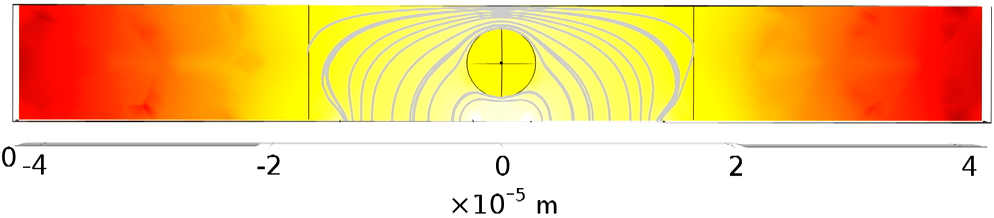
\includegraphics[width=\textwidth]{images/simple_cell_1Mhz.png}
        \caption{The electric field at 1 Mhz. Need to consider where membrane and cytoplasm relaxation occurs}
    \end{subfigure}
    \\
    \vspace{0.1 in}
    \begin{subfigure}[b]{\textwidth}
        \centering
        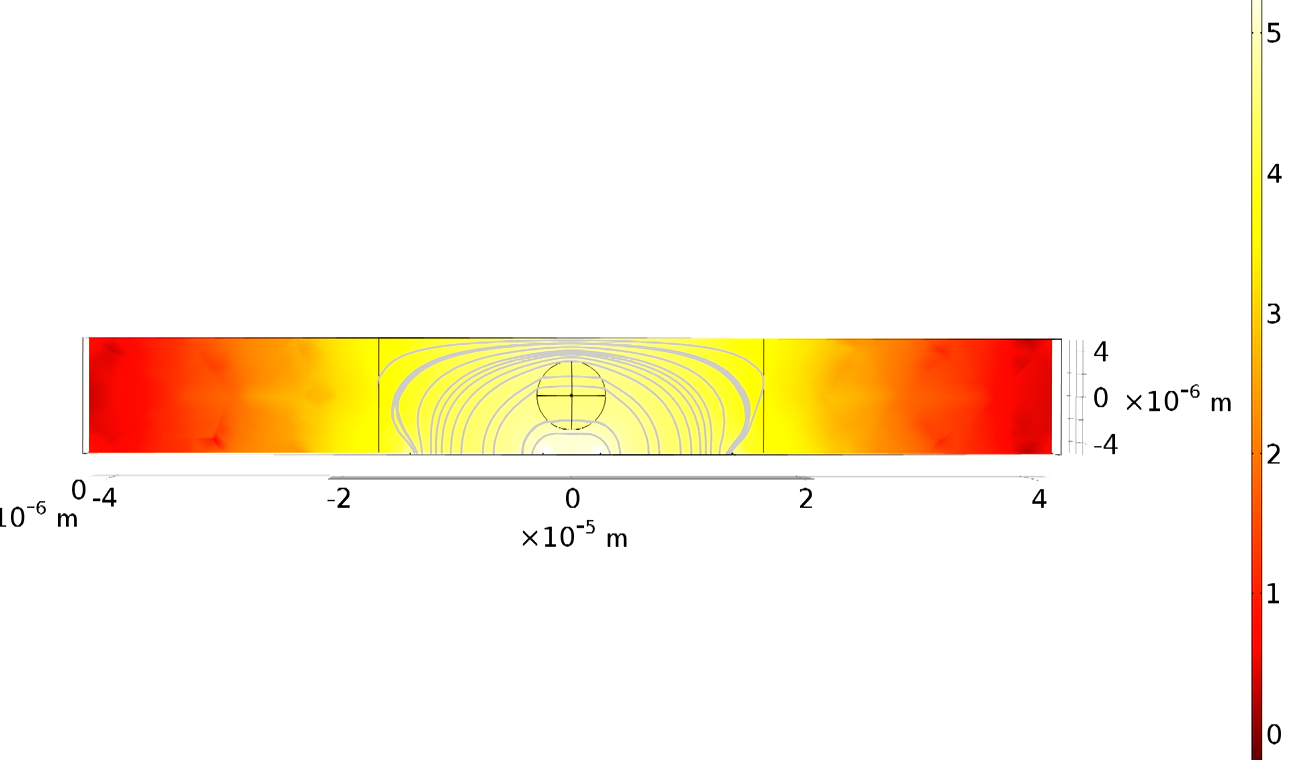
\includegraphics[width=\textwidth]{images/simple_cell_10Mhz.png}
        \caption{10 Mhz}
    \end{subfigure}
        \\
    \vspace{0.1 in}
    \begin{subfigure}[b]{\textwidth}
        \centering
        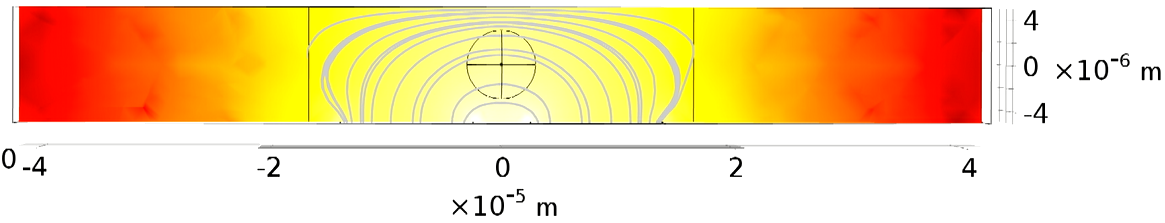
\includegraphics[width=\textwidth]{images/simple_cell_1Ghz.png}
        \caption{1 GHz}
    \end{subfigure}
        \\
    \vspace{0.1 in}
    \begin{subfigure}[b]{\textwidth}
        \centering
        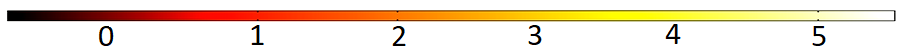
\includegraphics[width=\textwidth]{images/simpleCellColorMapAxis.png}
        \caption{The color map axis describing the logarithm of the magnitude of the electric field for the preceding sub-figures.}
    \end{subfigure}
    \caption[FEA simple model electric field surface plot.]{FEA simple model plots of the electric field at frequencies of interest. The logarithm of the electric field magnitude is depicted through the color mapping outlined by the color axis in sub-figure (e), and the electric field lines are illustrated with white curves in the region of the electrodes and cell.}
    \label{fig:single_cell_model_EZ_plots}
\end{figure}

\begin{figure}[h]
    \centering
    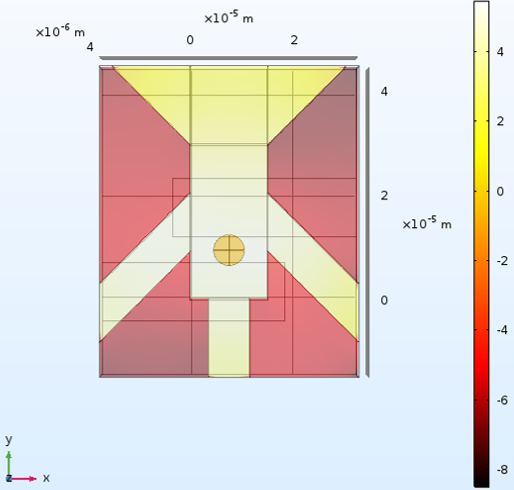
\includegraphics[width=0.7\textwidth]{images/deviceCellCurrent1Hz.png}
    \caption[Current density plot of the FEA device model.]{Current density plot of the FEA device model at DC. The color mapping depicts the logarithm of the current density magnitude.}
    \label{fig:device_current_denisty plot}
\end{figure}

Discuss the calculated device inefficiency.

\FloatBarrier

\subsection{optimization}

\begin{figure}[h]
    \centering
    \begin{subfigure}[b]{0.49\textwidth}
        \centering
        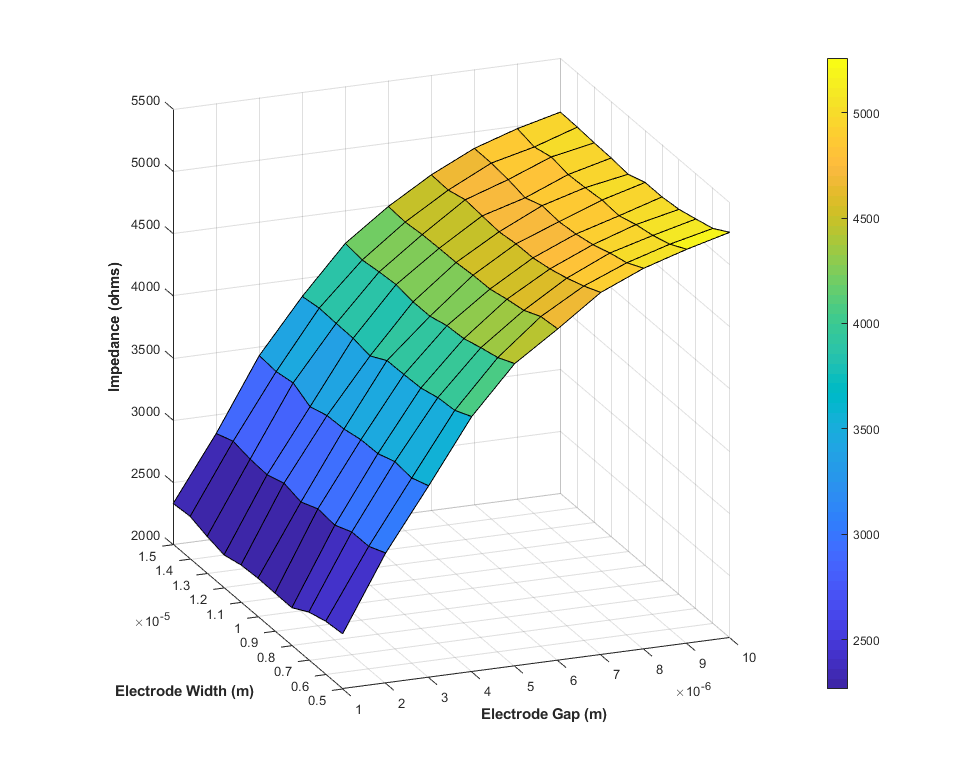
\includegraphics[width=\textwidth]{images/comsol_simple_difference.png}
        \caption{Difference}
    \end{subfigure}
    \hfill
    \begin{subfigure}[b]{0.49\textwidth}
        \centering
        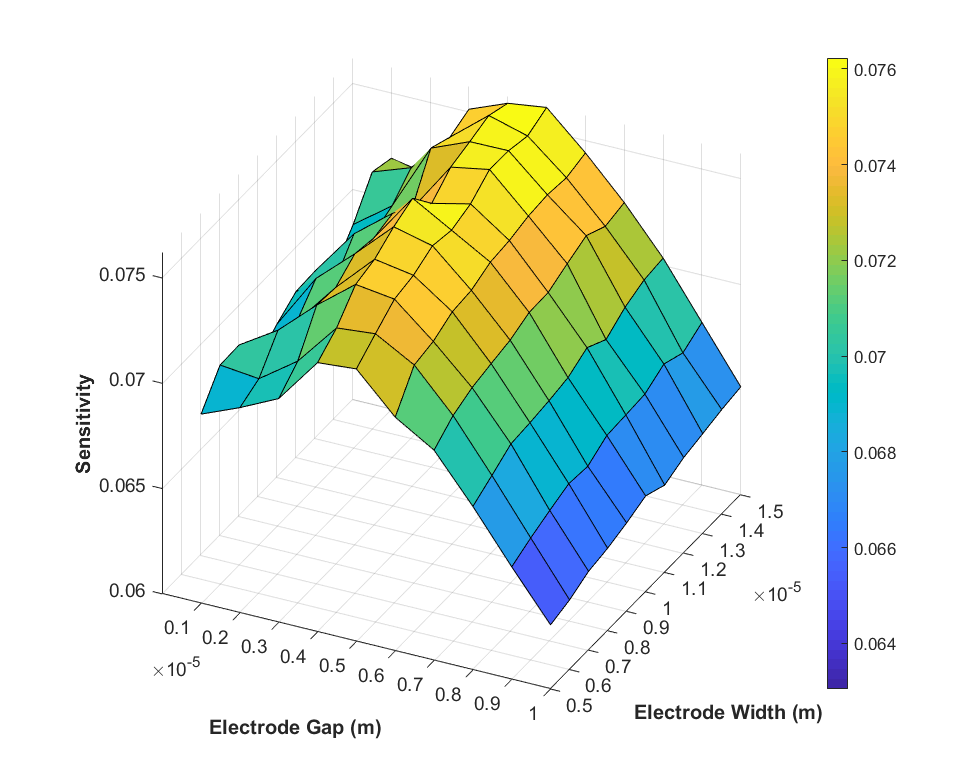
\includegraphics[width=\textwidth]{images/comsol_simple_sensitivity_surface.png}
        \caption{Sensitivity}
    \end{subfigure}
    \\
    \vspace{0.1 in}
    \begin{subfigure}[b]{0.49\textwidth}
        \centering
        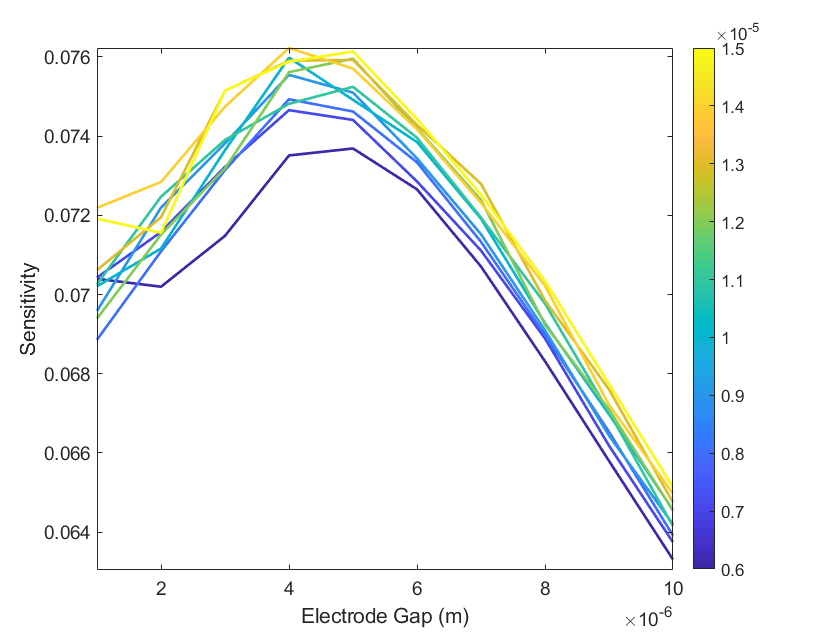
\includegraphics[width=\textwidth]{images/comsol_simple_gapXsensitivity.png}
        \caption{gap}
    \end{subfigure}
    \hfill
    \begin{subfigure}[b]{0.49\textwidth}
        \centering
        \includegraphics[width=\textwidth]{images/comsol_simple_widthXsensitivity.png}
        \caption{width}
    \end{subfigure}
    \caption[Simple sensitivity]{Simple sensitivity}
    \label{fig:simple_sensitivity}
\end{figure}

\begin{figure}[h]
    \centering
    \begin{subfigure}[b]{0.49\textwidth}
        \centering
        \includegraphics[width=\textwidth]{images/comsol_device_surface_difference.png}
        \caption{Difference}
    \end{subfigure}
    \hfill
    \begin{subfigure}[b]{0.49\textwidth}
        \centering
        \includegraphics[width=\textwidth]{images/comsol_device_surface_sensitivity.png}
        \caption{Sensitivity}
    \end{subfigure}
    \\
    \vspace{0.1 in}
    \begin{subfigure}[b]{0.49\textwidth}
        \centering
        \includegraphics[width=\textwidth]{images/comsol_device_gapXsensitivity.png}
        \caption{gap}
    \end{subfigure}
    \hfill
    \begin{subfigure}[b]{0.49\textwidth}
        \centering
        \includegraphics[width=\textwidth]{images/comsol_device_widthXsensitivity.png}
        \caption{width}
    \end{subfigure}
    \caption[Device sensitivity]{Device sensitivity}
    \label{fig:device_sensitivity}
\end{figure}

\begin{figure}[h]
    \centering
    \begin{subfigure}[b]{0.49\textwidth}
        \centering
        \includegraphics[width=\textwidth]{images/comsol_device_gapXsensitivity_aveError.png}
        \caption{Gap}
    \end{subfigure}
    \hfill
    \begin{subfigure}[b]{0.49\textwidth}
        \centering
        \includegraphics[width=\textwidth]{images/comsol_device_widthXsensitivity_aveError.png}
        \caption{Width}
    \end{subfigure}
    \caption[Device sensitivity average]{Device sensitivity average}
    \label{fig:device_sensitivity_average}
\end{figure}


\FloatBarrier

\section{Spice Model/Measurement analysis}
